\newif\ifglobal

%%%%%%%%%%%%%%%%%%%%%%%
%%% Compile to view %%%
%%%%%%%%%%%%%%%%%%%%%%%

%%%%%%%%%%%%%%%%%%%%%%%%%%%%%%%%%%%%%%%%%%%%%%%%%%%
%%% Readme:                                     %%%
%%% https://www.overleaf.com/read/bwdjvfjksvjy/ %%%
%%%%%%%%%%%%%%%%%%%%%%%%%%%%%%%%%%%%%%%%%%%%%%%%%%%

% >>> M?: marks a module setting number or important notice

% >>> M4: Set {./relative-path} to external files for this module <<<
\def \modulefiles {./10-PERMCTRL}
% To add an external file, use:
% (Replace '---' with actual filename)
% '\input{\modulefiles/tables/---.tex}' for tables
% '\includegraphics{\modulefiles/figures/---}' for figures
% '\subfile{\modulefiles/---}' for register files

% >>> M1: This module is in global project? <<<
% 'YES' - uncomment; 'NO' - comment out
\globaltrue

\ifglobal
    \documentclass[main\_\_CN.tex]{subfiles}

\else
    % Font "FandolSong-Regular" used by ctex does not have GSUB table.
    % It causes warnings that do not affect compilation and can be ignored.
    \PassOptionsToPackage{quiet}{fontspec}

    \documentclass[openany, 10pt]{book}

    % >>> M2: In ./00-shared/preamble-trm-module, also find
    %         settings for visibility of todo notes, watermark <<<
    \usepackage{preamble-trm-module}


    % Enable Chinese typesetting
    \usepackage{ctex}

    % >>> M3: Temporary labels in Chinese
    %         you can add your own labels there <<<
    \myexternaldocument{./00-shared/temp-labels-cn}

\fi %\ifglobal


\setcounter{secnumdepth}{4}

% >>> M5: If this module needs any updates in
% './00-shared/preamble-trm-module.sty'
% (include additional package, etc.), contact your module PM
% or create the file './00-shared/changelog.tex' make the
% necessary updates yourself and document them in this file <<<


\begin{document}


% Sets language into which pre-defined bits of text are translated
\selectlanguage{chinese}

% Do not delete this block
\ifglobal
% Add the following front matter if
% this module is outside of global project
\else
    \InputIfFileExists{readme}{}{}
    {\let\clearpage\relax \listoftodos}
    \tableofcontents
    \listoftables
    \listoffigures
\fi


%%%%%%%%%%%%%%%%%%%%%%%%%
%%% TRM Module Begins %%%
%%%%%%%%%%%%%%%%%%%%%%%%%

\hypertarget{permctrl}{}
\chapter{权限控制 (PMS)}
\label{mod:permctrl}

\section{概述}
\chipname{} 中所有的片内存储器、片外存储器、及外设均支持访问权限管理，CPU 必须拥有相应访问权限才能访问相应的从设备，从而保护数据和指令不被非法读取、改写和取指。

特别地，\chipname{} 允许用户使能 World 控制，将芯片的资源分为安全世界资源和非安全世界资源，CPU 处于不同世界时可以访问的权限不同，这部分内容请见章节 \ref{mod:wctrl} \textit{\nameref{mod:wctrl}}。本章节将主要介绍 \chipname{} 的权限管理机制及相关保护措施。



\section{主要特性}

\chipname{} 的权限控制具有以下特性：

\begin{itemize}
    \item 安全世界和非安全世界可独立配置
    \item 支持片内存储器的权限管理，包括：
    \begin{itemize}
        \item CPU 对片内存储器的访问权限控制
        \item CPU Trace 对片内存储器的访问权限控制
        \item GDMA 对片内存储器的访问权限控制
    \end{itemize}
    \item 支持片外存储器的权限管理
    \begin{itemize}
        \item SPI1 访问外部存储器的权限控制
        \item GDMA 访问外部存储器的权限控制
        \item CPU 通过 CACHE 访问外部存储器的权限控制
    \end{itemize}
    \item 支持外设的权限管理
    \begin{itemize}
        \item 绝大部份外设空间均支持独立的权限控制
        \item 支持非对齐访问的监测
        \item 支持自定义地址段权限管理
    \end{itemize}
    \item 内置权限寄存器锁保护机制
    \begin{itemize}
        \item 所有的权限寄存器都能够通过 lock 寄存器进行锁定，一旦权限寄存器被 lock 寄存器锁住，该权限寄存器以及 lock 寄存器都无法再次被修改，直到 CPU 复位才能解除锁定
    \end{itemize}
    \item 内置权限监测中断机制
    \item 内置 CPU 内部 VECBASE 寄存器覆盖机制
\end{itemize}

\section{片内存储器的权限管理}

\chipname{} 片内存储器的主要包括：
\begin{itemize}
    \item ROM：共 384 KB，分为 256 KB Internal ROM0 和 128 KB Internal ROM1。
    \item SRAM：共 512 KB，分为 32 KB Internal SRAM0、416 KB Internal SRAM1 和 64 KB Internal SRAM2。
    \item RTC 快速内存：共 8 KB，可由分割线分为高、低两个片区，各片区可独立配置权限。
    \item RTC 慢速内存：共 8 KB，可由分割线分为高、低两个片区，各片区可独立配置权限。
\end{itemize}
本节将依次介绍 \chipname{} 中有关片内存储资源访问权限管理。

\subsection{ROM 的访问权限管理}\label{sec:permctrl-PC-for-ROM}

\subsubsection{地址范围}

\chipname{} 的 ROM 允许 CPU 通过指令总线 IBUS 和数据总线 DBUS 进行访问，安全世界和非安全世界的权限可单独配置，但一旦配置对 CPU0 和 CPU1 同时生效，具体允许访问的地址空间范围请见下方表 \ref{tab:permctrl-ROM_block_address}。

\begin{table}[H]
    \centering
    \caption{ROM 地址范围}
    \label{tab:permctrl-ROM_block_address}

    \begin{tabular}{|*{5}{c|} }
    \hline
        \rowcolor{lightgray}
         & \multicolumn{2}{c|}{\textbf{IBUS 地址}} & \multicolumn{2}{c|}{\textbf{DBUS 地址}} \\\cline{2-5}
        \rowcolor{lightgray}
        \multirow{-2}*{\textbf{ROM}} & \textbf{起始地址} & \textbf{结束地址} & \textbf{起始地址} & \textbf{结束地址} \\\hline

        % table contents
        Internal ROM0  & 0x{}4000\_0000 & 0x{}4003\_FFFF & - & - \\\hline
        Internal ROM1  & 0x{}4004\_0000 & 0x{}4005\_FFFF & 0x{}3FF0\_0000 & 0x{}3FF1\_FFFF \\\hline
        \end{tabular}
    \end{table}

\subsubsection{权限配置}

\chipname{} 使用下方表 \ref{tab:permctrl-rom_permconfig} 中的寄存器，控制 CPU 的指令总线 (IBUS) 和数据总线 (DBUS) 从安全世界和非安全世界中对 ROM 的取指 (X)、写入 (W) 和读取 (R) 权限：

\begin{table}[H]
    \centering
    \caption{ROM 的权限配置}
    \label{tab:permctrl-rom_permconfig}
    \begin{threeparttable}
    \begin{tabular}{|l|l|l|l|}
        \hline
        \rowcolor{lightgray}
        \textbf{总线} & \textbf{所处的世界} & \textbf{ROM 权限配置寄存器\tnote{A}}                         & \textbf{权限设置顺序} \\ \hline
                     & 安全世界      & \hyperref[regdesc:PMSCOREXIRAM0PMSCONSTRAIN2REG]{PMS\_CORE\_X\_IRAM0\_PMS\_CONSTRAIN\_2\_REG   {[}20:18{]}} \tnote{B} & X/W/R           \\ \cline{2-4}
        \multirow{-2}{*}{IBUS} & 非安全世界 & \hyperref[regdesc:PMSCOREXIRAM0PMSCONSTRAIN1REG]{PMS\_CORE\_X\_IRAM0\_PMS\_CONSTRAIN\_1\_REG {[}20:18{]}}    & X/W/R \\ \hline
                     & 安全世界      & \hyperref[regdesc:PMSCOREXDRAM0PMSCONSTRAIN1REG]{PMS\_CORE\_X\_DRAM0\_PMS\_CONSTRAIN\_1\_REG   {[}25:24{]}}\tnote{C} & W/R             \\ \cline{2-4}
        \multirow{-2}{*}{DBUS} & 非安全世界 & \hyperref[regdesc:PMSCOREXDRAM0PMSCONSTRAIN1REG]{PMS\_CORE\_X\_DRAM0\_PMS\_CONSTRAIN\_1\_REG   {[}27:26{]}} & W/R   \\ \hline
        \end{tabular}
        \begin{tablenotes}
        \item[A] 配置为 1 表示具有对应权限，配置为 0 表示不具有对应权限。
        \item[B] 举例而言，配置该寄存器为 101 代表 CPU 的 IBUS 总线在安全世界中对 ROM 具有取指和读取权限，但没有写入权限。
        \item[C] 举例而言，配置该寄存器为 01 代表 CPU 的 DBUS 总线在安全世界中对 ROM 具有读取权限，但没有写入权限。
        \end{tablenotes}
     \end{threeparttable}
    \end{table}

\subsection{SRAM 的权限管理}

\subsubsection{地址范围}

\chipname{} 的 SRAM 允许 CPU 通过指令总线 IBUS 或数据总线 DBUS 进行访问，安全世界和非安全世界的权限可单独配置，但一旦配置对 CPU0 和 CPU1 同时生效，具体允许访问的地址空间范围请见下方表 \ref{tab:permctrl-SRAM_block_address}。

\begin{table}[H]
    \centering
    \caption{SRAM Block 地址范围}
    \label{tab:permctrl-SRAM_block_address}
    \begin{tabular}{ |*{6}{c|}}
    \hline
        \rowcolor{lightgray}
        & & \multicolumn{2}{c|}{\textbf{IBUS 地址}} & \multicolumn{2}{c|}{\textbf{DBUS 地址}} \\\cline{3-6}
        \rowcolor{lightgray}
        \multirow{-2}*{\textbf{SRAM}} & \multirow{-2}*{\textbf{Block}} & \textbf{起始地址} & \textbf{结束地址} & \textbf{起始地址} & \textbf{结束地址} \\\hline
        % table contents
        \multirow{2}*{Internal SRAM0}  & Block0 & 0x{}4037\_0000 & 0x{}4037\_3FFF & - & - \\\cline{2-6}
                                    & Block1 & 0x{}4037\_4000 & 0x{}4037\_7FFF & - & - \\\hline
    \multirow{7}*{Internal SRAM1}  & Block2 & 0x{}4037\_8000 & 0x{}4037\_FFFF & 0x{}3FC8\_8000 & 0x{}3FC8\_FFFF \\\cline{2-6}
                                    & Block3 & 0x{}4038\_0000 & 0x{}4038\_FFFF & 0x{}3FC9\_0000 & 0x{}3FC9\_FFFF \\\cline{2-6}
                                    & Block4 & 0x{}4039\_0000 & 0x{}4039\_FFFF & 0x{}3FCA\_0000 & 0x{}3FCA\_FFFF \\\cline{2-6}
                                    & Block5 & 0x{}403A\_0000 & 0x{}403A\_FFFF & 0x{}3FCB\_0000 & 0x{}3FCB\_FFFF \\\cline{2-6}
                                    & Block6 & 0x{}403B\_0000 & 0x{}403B\_FFFF & 0x{}3FCC\_0000 & 0x{}3FCC\_FFFF \\\cline{2-6}
                                    & Block7 & 0x{}403C\_0000 & 0x{}403C\_FFFF & 0x{}3FCD\_0000 & 0x{}3FCD\_FFFF \\\cline{2-6}
                                    & Block8 & 0x{}403D\_0000 & 0x{}403D\_FFFF & 0x{}3FCE\_0000 & 0x{}3FCE\_FFFF \\\hline
    \multirow{2}*{Internal SRAM 2}  & Block9 & - & - & 0x{}3FCF\_0000 & 0x{}3FCF\_7FFF \\\cline{2-6}
                                    & Block10 & - & - & 0x{}3FCF\_8000 & 0x{}3FCF\_FFFF \\\hline
        \end{tabular}
    \end{table}

本小节依次介绍了 Internal SRAM0、Internal SRAM1 和 Internal SRAM2 的权限配置。此外，还介绍了如何配置 Internal SRAM1 用作 Trace 内存。

\subsubsection{Internal SRAM0 的权限配置}\label{sec:permctrl_sram0}

\chipname{} 的 Internal SRAM0 分为 Block0 和 Block1（详见表 \ref{tab:permctrl-SRAM_block_address}），可分配给 CPU 或者 ICACHE 单独使用。一旦配置，对 CPU0 和 CPU1 同时生效。具体方式为配置如下表 \ref{tab:permctrl-sram0_accessconfig} 寄存器的对应位：

\begin{table}[H]
    \centering
    \caption{Internal SRAM0 的使用权限配置}
    \label{tab:permctrl-sram0_accessconfig}
    \begin{threeparttable}
    \begin{tabular}{|l|l|c|}
    \hline
    \rowcolor{lightgray}
                          &\textbf{Block}  & \textbf{\hyperref[regdesc:PMSINTERNALSRAMUSAGE1REG]{PMS\_INTERNAL\_SRAM\_USAGE\_1\_REG\tnote{A}}}\\\hline
    \multirow{2}{*}{SRAM} & Block0        & [0] \tnote{B}\\\cline{2-3}
                          & Block1        & [1] \\\hline
    \end{tabular}
    \begin{tablenotes}
        \item[A] 配置为 1 表示给 CPU 使用，配置为 0 表示给 ICACHE 使用。
        \item[B] 举例而言，配置该位为 1，表示将 SRAM 的 Block0 给 CPU 使用。
        \end{tablenotes}
    \end{threeparttable}
\end{table}

当 CPU 获得使用权限时，\chipname{} 使用下方表 \ref{tab:permctrl-sram0_permconfig} 中的寄存器，控制 CPU 的指令总线 (IBUS) 从安全世界和非安全世界中对 SRAM0 的取指 (X)、写入 (W) 和读取 (R) 权限：

\begin{table}[H]
    \centering
    \caption{Internal SRAM0 的访问权限配置}
    \label{tab:permctrl-sram0_permconfig}
    \begin{threeparttable}
    \begin{tabular}{ |l|l|l|l|l|l|}
    \hline
        \rowcolor{lightgray}
        & & & \multicolumn{2}{c|}{\textbf{SRAM0}} &  \\\cline{4-5}
        \rowcolor{lightgray}
        \multirow{-2}*{\textbf{总线\tnote{A}}}   & \multirow{-2}*{\textbf{所处的世界}} & \multirow{-2}*{\textbf{配置寄存器\tnote{B}}} & \textbf{Block0} & \textbf{Block1} & \multirow{-2}*{\textbf{权限设置顺序}} \\\hline
        % table contents
        \multirow{2}*{IBUS} & 安全世界   &
        \hyperref[regdesc:PMSCOREXIRAM0PMSCONSTRAIN2REG]{PMS\_CORE\_X\_IRAM0\_PMS\_CONSTRAIN\_2\_REG} & [14:12]\tnote{C} & [17:15] & X/W/R \\\cline{2-6}
                            & 非安全世界 & \hyperref[regdesc:PMSCOREXIRAM0PMSCONSTRAIN1REG]{PMS\_CORE\_X\_IRAM0\_PMS\_CONSTRAIN\_1\_REG} & [14:12] & [17:15] & X/W/R \\\hline
        \end{tabular}
        \begin{tablenotes}
            \item[A] CPU 必须同时拥有\hyperref[tab:permctrl-sram0_accessconfig]{使用权限}和访问权限才能访问 Internal SRAM0。
            \item[B] 配置为 1 表示具有对应权限，配置为 0 表示不具有对应权限。
            \item[C] 举例而言，配置该寄存器为 0b101 代表 CPU 的 IBUS 总线在安全世界中对 SRAM 的 Block0 具有取指和读取权限，没有写入权限。
        \end{tablenotes}
        \end{threeparttable}
    \end{table}

\subsubsection{Internal SRAM1 权限配置 }\label{sec:permctrl_sram1}

\chipname{} 的 Internal SRAM1 分为 Block2 \verb+~+ Block8（详见表 \ref{tab:permctrl-SRAM_block_address}）：
\begin{itemize}
    \item CPU 的数据总线 DBUS、指令总线 IBUS 和 GDMA 均可访问，且允许同时进行访问。
    \item 可用作 Trace 内存。
    \item 支持自定义地址段，可实现灵活的权限控制。
\end{itemize}


\chipname{} 允许用户通过 5 条分割线将 SRAM1 分割为 6 个自定义地址段，每个区域可以分别配置权限。

具体来说，Internal SRAM1 可由 IRam0\_DRam0\_split\_line 划分为指令空间和数据空间。
\begin{itemize}
    \item 指令空间 (Instruction Region)：
    \begin{itemize}
    \item 指令空间应配置为仅可由 IBUS 访问
    \item 且可以由 IRam0\_split\_line\_0 和 IRam0\_split\_line\_1 进一步划分为 3 个分割区域
    \end{itemize}
    \item 数据空间 (Data Region)：
    \begin{itemize}
        \item 数据空间应配置为仅可由 DBUS 访问
        \item 且可由 DRam0\_split\_line\_0 和 DRam0\_split\_line\_1 进一步划分为 3 个分割区域
    \end{itemize}
\end{itemize}

请见下方图 \ref{fig:permctrl_region_split} 和表 \ref{tab:permctrl_region_split} 所示。

\begin{figure}[!ht]
        \centering
        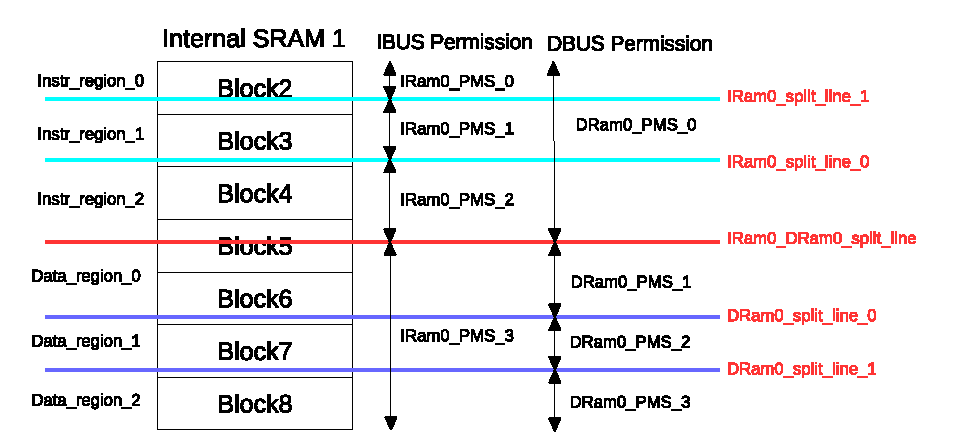
\includegraphics[width=0.7\textwidth]{./10-PERMCTRL/figures/pms_split_line.eps}
        \caption{Internal SRAM1 的区域分割示意图}
        \label{fig:permctrl_region_split}
    \end{figure}

具体请见下表：
\begin{table}[H]
\caption{Internal SRAM1 的区域分割}
\label{tab:permctrl_region_split}
\centering
\begin{threeparttable}
\begin{tabular}{|L{3cm}|L{6cm}|L{6cm}|}
\hline
\rowcolor{lightgray}
\textbf{内存}\tnote{A}                     & \textbf{空间}                                & \textbf{区域\tnote{B}}             \\ \hline
\multirow{6}{*}{SRAM1} & \multirow{3}{*}{Instruction Region} & Instr\_Region\_0 \\ \cline{3-3}
                       &                                     & Instr\_Region\_1 \\ \cline{3-3}
                       &                                     & Instr\_Region\_2 \\ \cline{2-3}
                       & \multirow{3}{*}{Data Region}      & Data\_Region\_0  \\ \cline{3-3}
                       &                                     & Data\_Region\_1  \\ \cline{3-3}
                       &                                     & Data\_Region\_2  \\ \hline
\end{tabular}
    \begin{tablenotes}
        \item[A] 各细分区域的权限可分别配置，请见下方表 \ref{tab:permctrl_sram1_inst_permsplit} 和 \ref{tab:permctrl_sram1_data_permsplit}。
        \item[B] 有关分割线的具体配置，请见下方的描述。
    \end{tablenotes}
\end{threeparttable}
\end{table}

\subparagraph{划分区域}\label{sec:permctrl-split-line}

\chipname{} 允许用户自行配置分割线的位置，每条分割线均有自己对应的配置寄存器。
\begin{itemize}
    \item 指令和数据空间分割线 IRam0\_DRam0\_split\_line 配置寄存器：
    \begin{itemize}
        \item \hyperref[regdesc:PMSCOREXIRAM0DRAM0DMASPLITLINECONSTRAIN1REG]{PMS\_CORE\_X\_IRAM0\_DRAM0\_DMA\_SPLIT\_LINE\_CONSTRAIN\_1\_REG}
    \end{itemize}
    \item 指令空间内部分割线 IRam0\_split\_line\_0  配置寄存器：
    \begin{itemize}
        \item \hyperref[regdesc:PMSCOREXIRAM0DRAM0DMASPLITLINECONSTRAIN2REG]{PMS\_CORE\_X\_IRAM0\_DRAM0\_DMA\_SPLIT\_LINE\_CONSTRAIN\_2\_REG}
    \end{itemize}
    \item 指令空间内部分割线 IRam0\_split\_line\_1  配置寄存器：
    \begin{itemize}
        \item \hyperref[regdesc:PMSCOREXIRAM0DRAM0DMASPLITLINECONSTRAIN3REG]{PMS\_CORE\_X\_IRAM0\_DRAM0\_DMA\_SPLIT\_LINE\_CONSTRAIN\_3\_REG}
    \end{itemize}
    \item 数据空间内部分割线 DRam0\_split\_line\_0  配置寄存器：
    \begin{itemize}
        \item \hyperref[regdesc:PMSCOREXIRAM0DRAM0DMASPLITLINECONSTRAIN4REG]{PMS\_CORE\_X\_IRAM0\_DRAM0\_DMA\_SPLIT\_LINE\_CONSTRAIN\_4\_REG}
    \end{itemize}
    \item 数据空间内部分割线 DRam0\_split\_line\_1  配置寄存器：
    \begin{itemize}
        \item \hyperref[regdesc:PMSCOREXIRAM0DRAM0DMASPLITLINECONSTRAIN5REG]{PMS\_CORE\_X\_IRAM0\_DRAM0\_DMA\_SPLIT\_LINE\_CONSTRAIN\_5\_REG}
    \end{itemize}
\end{itemize}

\begin{figure}[!ht]
        \centering
        
\includegraphics[width=0.5\textwidth]{./10-PERMCTRL/figures/split_line_category.eps}
        \caption{分割线 Category 分配示意图}
        \label{fig:PERMCTRL_category_config}
\end{figure}

每条分割线在配置时应：
\begin{enumerate}
    \item 首先配置分割线所处的 Block：
    \begin{itemize}
        \item 将分割线所处 Block 对应的 Category\_\regindex{x} 域配置为 0x{}1 或者 0x{}2（没有区别）；
        \item 之前所有 Block 对应的 Category\_0 \verb+~+ Category\_\regindex{x-1} 域全被配置为 0x{}0；
        \item 之后所有 Block 对应的 Category\_\regindex{x+1} \verb+~+ Category\_6 域全部配置为 0x{}3。
    \end{itemize}
        举例而言，假设分割线位于 Block5，则应将 Block5 对应的 Category\_3 域配置为 0x{}1 或者 0x{}2；将 Block2 \verb+~+ Block4 对应的 Category\_0 \verb+~+ Category\_2 域全部配置为 0x{}0；将 Block6 \verb+~+ Block8 对应的 Category\_4 \verb+~+ Category\_6 域全部配置为 0x{}3。可参考图 \ref{fig:PERMCTRL_category_config}。反过来，查询到 Category\_3 域为 0x{}1 或者 0x{}2 也可以了解分割线处于 Block5。
    \item 配置分割线在所处 Block 中的位置：
    \begin{itemize}
        \item 将需要分割的 IBUS 或 DBUS 访问地址的 [15:8] 位写入分割线对应配置寄存器的 \hyperref[fielddesc:PMSCOREXIRAM0SRAMLINE0SPLITADDR]{SPLITADDR} 域中。
        \item 注意分割地址必须配置为与 256 Byte 对齐，也就是说必须是 0x{}100 的整数倍。
    \end{itemize}
        举例而言，假设需要分割的 IBUS 地址为 0x{}3fc88000，则应将该地址的 [15:8] 位，即 0b10000000 写入该分割线对应配置寄存器的 \hyperref[fielddesc:PMSCOREXIRAM0SRAMLINE0SPLITADDR]{SPLITADDR} 域。
\end{enumerate}

值得注意的是，用户在配置 5 条分割线时还应遵循以下原则：

 \begin{itemize}
     \item 位置要求
     \begin{itemize}
         \item 指令和数据空间分割线可以配置为 SRAM1 的任何位置
         \item 指令空间中的 2 条内部分割线不能超出指令空间，相对位置无要求。
         \item 数据空间中的 2 条内部分割线不能超出数据空间，相对位置无要求。
     \end{itemize}
     \item 各分割线可以相互重合，相当于不存在。举例而言：
     \begin{itemize}
         \item 数据空间中的 2 条内部分隔线如果不重合，则相当于将数据空间分为 3 个细分区域；
         \item 数据空间中的 2 条内部分隔线如果重合，则相当于仅将数据空间分为 2 个细分区域；
         \item 数据空间中的 2 条内部分隔线如果本身 两两重合，且与指令和数据空间分割线重合，则相当于对数据空间内部不做细分，仅有一个数据空间区域.
     \end{itemize}
     \end{itemize}

\subparagraph{配置权限}

完成对分割线的配置后，用户可通过下表中的寄存器，独立配置 CPU 的 IBUS、DBUS 和 GDMA 外设从不同世界中，对细分指令空间和数据空间的访问权限。

对细分指令空间的配置如表 \ref{tab:permctrl_sram1_inst_permsplit} 所示：

\begin{table}[H]
    \centering
    \caption{Internal SRAM1 的访问权限控制 -- 指令空间}
    \label{tab:permctrl_sram1_inst_permsplit}

    \begin{threeparttable}
    \begin{tabular}{ |l|l|l|c|c|c|l| }
    \hline
    \rowcolor{lightgray}
        & & & \multicolumn{3}{c|}{\textbf{指令空间}} &  \\\cline{4-6}
    \rowcolor{lightgray}
    \multirow{-2}*{\textbf{总线}}   & \multirow{-2}*{\textbf{所处的世界}} & \multirow{-2}*{\textbf{配置寄存器}} & \scriptsize{\textbf{instr\_region\_0}} & \scriptsize{\textbf{instr\_region\_1}} & \scriptsize{\textbf{instr\_region\_2}} & \multirow{-2}*{\textbf{权限设置顺序}}   \\\hline
    \multirow{2}*{IBUS}             & 安全世界        & \scriptsize{\hyperref[regdesc:PMSCOREXIRAM0PMSCONSTRAIN2REG]{PMS\_CORE\_X\_IRAM0\_PMS\_CONSTRAIN\_2\_REG}} & [2:0] & [5:3] & [8:6] & X/W/R \\\cline{2-7}
                                    & 非安全世界      & \scriptsize{\hyperref[regdesc:PMSCOREXIRAM0PMSCONSTRAIN1REG]{PMS\_CORE\_X\_IRAM0\_PMS\_CONSTRAIN\_1\_REG}} & [2:0] & [5:3] & [8:6] & X/W/R \\\hline

     \multirow{2}*{DBUS}            & 安全世界        &                                                                             & \multicolumn{3}{c|}{[1:0]\tnote{A}} & W/R \\ \cline{2-2} \cline{4-7}
                                    & 非安全世界      & \multirow{-2}*{\scriptsize{\hyperref[regdesc:PMSCOREXDRAM0PMSCONSTRAIN1REG]{PMS\_Core\_X\_DRAM0\_PMS\_CONSTRAIN\_1\_REG}}}      & \multicolumn{3}{c|}{[13:11]\tnote{A}}  & W/R \\\hline
    GDMA                        & \regindex{XX} 外设 \tnote{C}             & \scriptsize{\hyperref[regdesc:PMSDMAAPBPERISPI2PMSCONSTRAIN1REG]{PMS\_DMA\_APBPERI\_\regindex{XX}\_PMS\_CONSTRAIN\_1\_REG}}  &   \multicolumn{3}{c|}{[1:0]\tnote{B}}   & W/R \\\hline

    \end{tabular}
        \begin{tablenotes}
            \item [A] 可配置 DBUS 数据总线在指令空间中的访问权限，但建议将 DBUS 对指令空间的权限配置为 0。
            \item [B] 可配置 GDMA 在指令空间中的访问权限，但建议将 GDMA 对指令空间的权限配置为 0。
            \item [C] \chipname{} 共有 9 个外设（分别为 SPI2、SPI3、UCHI0、I2S0、I2S1、AES、SHA、ADC、LCD\_CAM、USB、SDIO\_HOST、RMT）可通过 GDMA 访问 Internal SRAM 1，所有的外设都有独立的权限寄存器控制其访问权限。
        \end{tablenotes}
     \end{threeparttable}
    \end{table}

对细分数据空间的配置如表 \ref{tab:permctrl_sram1_data_permsplit} 所示：


\begin{table}[H]
    \centering
    \caption{Internal SRAM1 的访问权限控制 -- 数据空间}
    \label{tab:permctrl_sram1_data_permsplit}

    \begin{threeparttable}
    \begin{tabular}{ |l|l|l|c|c|c|l| }
    \hline
    \rowcolor{lightgray}
        & & & \multicolumn{3}{c|}{\textbf{数据空间}} &  \\\cline{4-6}
    \rowcolor{lightgray}
    \multirow{-2}*{\textbf{总线}}   & \multirow{-2}*{\textbf{所处的世界}} & \multirow{-2}*{\textbf{配置寄存器}} & \scriptsize{\textbf{data\_region\_0}} & \scriptsize{\textbf{data\_region\_1}} & \scriptsize{\textbf{data\_region\_2}} & \multirow{-2}*{\textbf{权限设置顺序}}   \\\hline
     \multirow{2}*{IBUS}            & 安全世界        &    \scriptsize{\hyperref[regdesc:PMSCOREXIRAM0PMSCONSTRAIN2REG]{PMS\_CORE\_X\_IRAM0\_PMS\_CONSTRAIN\_2\_REG}}   & \multicolumn{3}{c|}{[11:9]\tnote{A}}  & X/W/R \\ \cline{2-7}
                                    & 非安全世界      & \scriptsize{\hyperref[regdesc:PMSCOREXIRAM0PMSCONSTRAIN1REG]{PMS\_CORE\_X\_IRAM0\_PMS\_CONSTRAIN\_1\_REG}}      & \multicolumn{3}{c|}{[11:9]\tnote{A}}  & X/W/R \\\hline
    \multirow{2}*{DBUS}             & 安全世界        &                                                                                    & [3:2] & [5:4] & [7:6] & W/R \\\cline{2-2} \cline{4-7}
                                    & 非安全世界      & \multirow{-2}*{\scriptsize{\hyperref[regdesc:PMSCOREXDRAM0PMSCONSTRAIN1REG]{PMS\_Core\_X\_DRAM0\_PMS\_CONSTRAIN\_1\_REG}}} & [15:14] & [17:16] & [19:18] & W/R \\\hline
    GDMA                    & \regindex{XX} 外设\tnote{B}              & \scriptsize{\hyperref[regdesc:PMSDMAAPBPERISPI2PMSCONSTRAIN1REG]{PMS\_DMA\_APBPERI\_\regindex{XX}\_PMS\_CONSTRAIN\_1\_REG}}  &  [3:2] & [5:4] & [7:6]    & W/R \\\hline

    \end{tabular}
        \begin{tablenotes}
            \item [A] 可配置 IBUS 指令总线在数据空间中的访问权限，但建议将 IBUS 对数据空间的权限配置为 0。
            \item [B] \chipname{} 共有 9 个外设（分别为 SPI2、SPI3、UCHI0、I2S0、I2S1、AES、SHA、ADC、LCD\_CAM、USB、SDIO\_HOST、RMT）可通过 GDMA 访问 Internal SRAM 1，所有的外设都有独立的权限寄存器控制其访问权限。
            \end{tablenotes}
     \end{threeparttable}
\end{table}

有关分割线的具体配置，请见第 \ref{sec:permctrl-split-line}。

\subparagraph{Trace 内存} \label{sec:permctrl_trace}
\chipname{} 搭载低功耗 Xtensa LX7 32 位双核处理器，内置 TRAX (Real-time Trace) 压缩模块，可便利开发人员的调试。该模块的实现需要 16 KB 存储空间，用户可从 Internal SRAM1 中分配 16 KB 用作 Trace 记录存储器，CPU0 和 CPU1 可分别配置。


用户可通过配置 \hyperref[regdesc:PMSINTERNALSRAMUSAGE2REG]{PMS\_INTERNAL\_SRAM\_USAGE\_2\_REG} 寄存器从 Internal SRAM1 中选择 16 KB 作为 Trace Memory，详细步骤如下所示。

\begin{enumerate}
    \item 首先，配置 \hyperref[fielddesc:PMSINTERNALSRAMCORE0TRACEUSAGE]{PMS\_INTERNAL\_SRAM\_CORE\regindex{m}\_TRACE\_USAGE} 域中各 Block 对应的位为 1 选择 Block：
    \begin{itemize}
        \item Block2: 0b00000001
        \item Block3: 0b00000010
        \item Block4: 0b00000100
        \item Block5: 0b00001000
        \item Block6: 0b00010000
        \item Block7: 0b00100000
        \item Block8: 0b01000000
    \end{itemize}
    \item 其次，配置  \hyperref[fielddesc:PMSINTERNALSRAMCORE0TRACEALLOC]{PMS\_INTERNAL\_SRAM\_CORE\regindex{m}\_TRACE\_ALLOC} 域，从选中的 Block 中选择 16 KB
    \begin{itemize}
        \item 2'b00：第一个 16 KB
        \item 2'b01：第二个 16 KB
        \item 2'b10：第三个 16 KB
        \item 2'b11：第四个 16 KB
    \end{itemize}
    注意，Block2 仅有 32 KB，因此如在第一步选择 Block2 则这里仅可配置为 2'b00 或 2'b0。
\end{enumerate}

举例而言，假设你希望配置 Internal SRAM1 中 Block3 的第一个 16 KB 作为 CPU0 的 Trace memory, 则需要
\begin{itemize}
    \item 配置 \hyperref[fielddesc:PMSINTERNALSRAMCORE0TRACEUSAGE]{PMS\_INTERNAL\_SRAM\_CORE0\_TRACE\_USAGE} 域为 0b0000010，选择 Block3
    \item 配置 \hyperref[fielddesc:PMSINTERNALSRAMCORE0TRACEALLOC]{PMS\_INTERNAL\_SRAM\_CORE0\_TRACE\_ALLOC} 域为 2'b00，选择第一个 16 KB。
\end{itemize}

\subsubsection{Internal SRAM2 权限配置}\label{sec:permctrl_sram2}

\chipname{} 的 Internal SRAM2 分为 Block9 和 Block10（详见表 \ref{tab:permctrl-SRAM_block_address}），可分配给 CPU/GDMA 或者 DCACHE 单独使用。一旦配置，对 CPU0 和 CPU1 同时生效。具体方式为配置如下表 \ref{tab:permctrl-sram2_accessconfig} 寄存器的对应位：

\begin{table}[H]
    \centering
    \caption{Internal SRAM2 的使用权限配置}
    \label{tab:permctrl-sram2_accessconfig}
    \begin{threeparttable}
    \begin{tabular}{|l|l|c|}
    \hline
    \rowcolor{lightgray}
                          &\textbf{Block}  & \textbf{\hyperref[regdesc:PMSINTERNALSRAMUSAGE1REG]{PMS\_INTERNAL\_SRAM\_USAGE\_1\_REG}\tnote{A}}\\\hline
    \multirow{2}{*}{SRAM} & Block9        & [3]\tnote{B} \\\cline{2-3}
                          & Block10        & [2] \\\hline
    \end{tabular}
        \begin{tablenotes}
        \item[A] 配置为 1 表示给 CPU 和 GDMA 使用，配置为 0 表示给 DCACHE 使用。
        \item[B] 举例而言，配置该位为 1，表示将 SRAM 的 Block9 给 CPU 和 GDMA 使用。
        \end{tablenotes}
    \end{threeparttable}
\end{table}

当 CPU 和 GDMA 获得使用权限时，\chipname{} 使用下方表 \ref{tab:permctrl-SRAM2_block_address} 中的寄存器，控制 CPU 的数据总线 (DBUS) 在不同世界中对 SRAM2 的写入 (W) 和读取 (R) 权限：

\begin{table}[H]
    \centering
    \caption{Internal SRAM2 的访问权限配置}
    \label{tab:permctrl-SRAM2_block_address}
    \begin{threeparttable}
    \begin{tabular}{ |l|l|l|l|l|l|}
    \hline
        \rowcolor{lightgray}
        & & & \multicolumn{2}{c|}{\textbf{SRAM2}} &  \\\cline{4-5}
        \rowcolor{lightgray}
        \multirow{-2}*{\textbf{总线 \tnote{A}}}   & \multirow{-2}*{\textbf{所处的世界}} & \multirow{-2}*{\textbf{配置寄存器}} & \textbf{Block9} & \textbf{Block10} & \multirow{-2}*{\textbf{权限设置顺序}\tnote{B}} \\\hline
        % table contents
        \multirow{2}*{DBUS} & 安全世界   & \hyperref[regdesc:PMSCOREXDRAM0PMSCONSTRAIN1REG]{PMS\_CORE\_X\_DRAM0\_PMS\_CONSTRAIN\_1\_REG}& [9:8]\tnote{C} & [11:10] & W/R \\\cline{2-6}
                            & 非安全世界 & \hyperref[regdesc:PMSCOREXDRAM0PMSCONSTRAIN1REG]{PMS\_CORE\_X\_DRAM0\_PMS\_CONSTRAIN\_1\_REG} & [21:20] & [23:22] & W/R \\\hline
        GDMA                    & \regindex{XX} 外设\tnote{B}              & \hyperref[regdesc:PMSDMAAPBPERISPI2PMSCONSTRAIN1REG]{PMS\_DMA\_APBPERI\_\regindex{XX}\_PMS\_CONSTRAIN\_1\_REG}  &  [9:8] & [11:10]    & W/R \\\hline
        \end{tabular}
        \begin{tablenotes}
            \item[A] CPU 和 GDMA 必须同时拥有使用权限和访问权限才能访问 Internal SRAM2。
            \item[B] 配置为 1 表示具有对应权限，配置为 0 表示不具有对应权限。
            \item[C] 举例而言，配置该寄存器为 0b10 代表 CPU 和 GDMA 的 DBUS 总线在安全世界中对 SRAM 的 Block9 具有写入权限，但没有读取权限。
        \end{tablenotes}
        \end{threeparttable}
    \end{table}

\subsection{RTC 快速内存 (FAST Memory) 的权限管理}

\subsubsection{地址范围}

\chipname{} 的 RTC FAST Memory 的存储空间大小为 8 KB，访问地址范围如下：

\begin{longtable}[c]{ |c|l|l| }
\caption{地址范围}
\label{tab:fast-memory-address}
\\\hline
\rowcolor{lightgray}
    \textbf{内存} &  \textbf{起始地址}  &  \textbf{结束地址}\\
    \hline
    RTC 快速内存           & 0x{}600F\_E000 &  0x{}600F\_FFFF   \\
    \hline
\end{longtable}

\subsubsection{权限配置}
为了实现更细化的权限管理，\chipname{} 允许用户使用 1 条分割线将 RTC 快速存储空间分割为 2 个区域。用户可通过配置相应寄存器（\hyperref[regdesc:PMSCORE0PIFPMSCONSTRAIN1REG]{PMS\_CORE\_\regindex{m}\_PIF\_PMS\_CONSTRAN\_\regindex{n}\_REG}），独立配置 CPU0 和 CPU1 在安全世界和非安全世界中的分割线及分割区域权限。

分割线的配置如下表所示：
\begin{table}[H]
    \centering
    \caption{RTC 快速内存的分割}
    \label{tab:rtc_fast_mem_split}
    \begin{threeparttable}
    \begin{tabular}{|l|l|l|} \hline
    \rowcolor{lightgray}
     & \multicolumn{2}{c|}{\textbf{分割地址配置寄存器}\tnote{1}} \\\cline{2-3}
    \rowcolor{lightgray}
    \multirow{-2}*{\textbf{RTC 快速内存}}  & \textbf{安全世界} & \textbf{非安全世界} \\\hline
    高地址段 &                   &       \\\cline{1-1}
    低地址段 & \multirow{-2}*{\hyperref[regdesc:PMSCORE0PIFPMSCONSTRAIN9REG]{PIF\_PMS\_CONSTRAN\_9\_REG} [10:0]}  & \multirow{-2}*{\hyperref[regdesc:PMSCORE0PIFPMSCONSTRAIN9REG]{PIF\_PMS\_CONSTRAN\_9\_REG} [21:11]} \\\hline
    \end{tabular}
        \begin{tablenotes}
        \item[1] 分割地址应采用相对于 RTC 快速内存基地址的偏移量。举例而言，用户如需设置 0x{}600F\_F000 作为分割线地址，则应配置此寄存器为 0x{}1000 的字地址。
        \end{tablenotes}
    \end{threeparttable}
\end{table}

各地址段的权限配置如下表所示：
\begin{table}[H]
    \centering
    \caption{RTC 快速内存的权限配置}
    \label{tab:rtc_fast_mem_split_access}
    \begin{threeparttable}
    \begin{tabular}{|l|l|l|l|l|} \hline
    \rowcolor{lightgray}
     & & \multicolumn{2}{c|}{\textbf{权限配置寄存器}}& \\\cline{3-4}
    \rowcolor{lightgray}
    \multirow{-2}*{\textbf{总线}}   & \multirow{-2}*{\textbf{RTC 快速内存}}  & \textbf{安全世界} & \textbf{非安全世界} & \multirow{-2}*{\textbf{配置顺序}\tnote{A}} \\\hline
     外设总线    & 高地址段                       &   \hyperref[regdesc:PMSCORE0PIFPMSCONSTRAIN10REG]{PIF\_PMS\_CONSTRAN\_10\_REG} [5:3] \tnote{B}               &    \hyperref[regdesc:PMSCORE0PIFPMSCONSTRAIN10REG]{PIF\_PMS\_CONSTRAN\_10\_REG} [11:9]  & \\\cline{2-4}
      (PIF)& 低地址段 & \hyperref[regdesc:PMSCORE0PIFPMSCONSTRAIN10REG]{PIF\_PMS\_CONSTRAN\_10\_REG} [2:0] & \hyperref[regdesc:PMSCORE0PIFPMSCONSTRAIN10REG]{PIF\_PMS\_CONSTRAN\_10\_REG} [8:6]  & \multirow{-2}*{X/W/R}  \\\hline
    \end{tabular}
        \begin{tablenotes}
        \item[A] 配置为 1 表示具有对应权限，配置为 0 表示不具有对应权限。
        \item[B] 举例而言，配置该寄存器为 101 代表 CPU 的 PIF 外设总线在安全世界中对 RTC 快速内存的高地址段有取指和读取权限，但没有写入权限。
        \end{tablenotes}
    \end{threeparttable}
\end{table}

\subsection{RTC 慢速内存 (SLOW Memory) 的权限管理}

\subsubsection{地址范围}

\chipname{} 的 RTC 慢速内存总大小为 8 KB。这块内存允许用户使用两套地址访问，详情见下方表 \ref{tab:slow-memory-address}：

\begin{longtable}[c]{ |c|l|l| }
\caption{地址范围}
\label{tab:slow-memory-address}
\\\hline
\rowcolor{lightgray}
    \textbf{RTC SLOW Memory} &  \textbf{起始地址}  &  \textbf{结束地址}\\
    \hline
    RTCSlow\_0           & 0x{}5000\_0000 &  0x{}5000\_1FFF   \\
    \hline
    RTCSlow\_1           & 0x{}6002\_1000 &  0x{}6002\_2FFF   \\
    \hline
\end{longtable}

\subsubsection{权限配置}

为了实现更细化的权限管理，\chipname{} 允许用户使用 2 条分割线分别将上述 2 个存储空间分别分割为 2 个区域。用户可通过配置相应寄存器（\hyperref[regdesc:PMSCORE0PIFPMSCONSTRAIN1REG]{PMS\_CORE\_\regindex{m}\_PIF\_PMS\_CONSTRAN\_\regindex{n}\_REG}），独立配置 CPU0 和 CPU1 在安全世界和非安全世界中的分割线及分割区域权限。

分割线的配置如下表所示：
\begin{table}[H]
    \centering
    \caption{RTC 慢速内存的分割}
    \label{tab:rtc_slow_mem_split}
    \begin{threeparttable}
    \begin{tabular}{|l|l|l|} \hline
    \rowcolor{lightgray}
    & \multicolumn{2}{c|}{\textbf{分割地址配置寄存器}\tnote{1}} \\\cline{2-3}
    \rowcolor{lightgray}
    \multirow{-2}*{\textbf{RTC 慢速内存}}  & \textbf{安全世界} & \textbf{非安全世界} \\\hline
    RTCSlow\_0 高地址段 &                   &       \\\cline{1-1}
    RTCSlow\_0 低地址段 & \multirow{-2}*{\hyperref[regdesc:PMSCORE0PIFPMSCONSTRAIN11REG]{PIF\_PMS\_CONSTRAN\_11\_REG} [10:0]}  & \multirow{-2}*{\hyperref[regdesc:PMSCORE0PIFPMSCONSTRAIN9REG]{PIF\_PMS\_CONSTRAN\_9\_REG} [21:11]} \\\hline
    RTCSlow\_1 高地址段 &                   &       \\\cline{1-1}
    RTCSlow\_1 低地址段 & \multirow{-2}*{\hyperref[regdesc:PMSCORE0PIFPMSCONSTRAIN13REG]{PIF\_PMS\_CONSTRAN\_13\_REG} [10:0]}  & \multirow{-2}*{\hyperref[regdesc:PMSCORE0PIFPMSCONSTRAIN13REG]{PIF\_PMS\_CONSTRAN\_13\_REG} [21:11]} \\\hline
    \end{tabular}
        \begin{tablenotes}
        \item[1] 分割地址应采用相对于 RTC 慢速内存基地址的偏移量。举例而言，用户如需设置 0x{}6002\_2000 作为分割线地址，则应配置此寄存器为 0x{}1000 的地址。
        \end{tablenotes}
    \end{threeparttable}
\end{table}

\begin{table}[H]
    \centering
    \caption{RTC 慢速内存的权限管理}
    \label{tab:rtc_slow1_mem_pms}
    \begin{threeparttable}
    \begin{tabular}{ | l | l | l | l | L{1cm} |}
    \hline
        \rowcolor{lightgray}
        & & \multicolumn{2}{c|}{\textbf{权限配置}} &  \textbf{配置}\tnote{A} \\\cline{3-4}
        \rowcolor{lightgray}
        \multirow{-2}*{\textbf{总线}}  & \multirow{-2}*{\textbf{RTC 慢速内存}} & \textbf{安全世界} & \textbf{安全世界} & \textbf{顺序} \\\hline

        外设 & RTCSlow\_0 高地址段 & \hyperref[regdesc:PMSCORE0PIFPMSCONSTRAIN12REG]{PIF\_PMS\_CONSTRAN\_12\_REG} [5:3]\tnote{B} & \hyperref[regdesc:PMSCORE0PIFPMSCONSTRAIN12REG]{PIF\_PMS\_CONSTRAN\_12\_REG} [11:9] & \\\cline{2-4}
        总线  & RTCSlow\_0 低地址段 & \hyperref[regdesc:PMSCORE0PIFPMSCONSTRAIN12REG]{PIF\_PMS\_CONSTRAN\_12\_REG} [2:0] & \hyperref[regdesc:PMSCORE0PIFPMSCONSTRAIN12REG]{PIF\_PMS\_CONSTRAN\_12\_REG} [8:6] & \\\cline{2-4}
        (PIF)& RTCSlow\_1 高地址段 & \hyperref[regdesc:PMSCORE0PIFPMSCONSTRAIN14REG]{PIF\_PMS\_CONSTRAN\_14\_REG} [5:3] & \hyperref[regdesc:PMSCORE0PIFPMSCONSTRAIN14REG]{PIF\_PMS\_CONSTRAN\_14\_REG} [11:9] & \\\cline{2-4}
          & RTCSlow\_1 低地址段 & \hyperref[regdesc:PMSCORE0PIFPMSCONSTRAIN14REG]{PIF\_PMS\_CONSTRAN\_14\_REG} [2:0] & \hyperref[regdesc:PMSCORE0PIFPMSCONSTRAIN14REG]{PIF\_PMS\_CONSTRAN\_14\_REG} [8:6] & \multirow{-4}*{X/W/R} \\\hline

        \end{tabular}

        \begin{tablenotes}
        \item[A] 权限设置顺序为 X/W/R。如访问权限与配置权限不一致时，则访问将被拒绝，具体表现为取指和读取操作仅能得到 0，写入操作失败。
        \item[B] 举例而言，配置该寄存器为 0b100 代表 CPU 的 PIF 外设总线从安全世界中对 RTC Slow\_0 的高地址段仅有取指权限，没有写入或读取权限。
        \end{tablenotes}
    \end{threeparttable}
\end{table}

\section{外设权限管理}
\subsection{外设空间权限控制}\label{sec:permctrl-peri-address}

\chipname{} 的模块和外设的权限大多均可独立控制，仅有部分外设共用一套权限管理寄存器，详见下表 \ref{tab:permctrl-peripheral-controlling-bit}。
用户可通过配置相应寄存器（\hyperref[regdesc:PMSCORE0PIFPMSCONSTRAIN1REG]{PMS\_CORE\_\regindex{m}\_PIF\_PMS\_CONSTRAN\_\regindex{n}\_REG}），独立配置 CPU0 和 CPU1 在安全世界和非安全世界中对相应模块或外设的读写权限（从高到低为 R/W）。当 CPU 对外设发起的访问类型与所配置类型不一致时，该访问将被拒绝，具体表现为读操作仅能得到 0，写操作直接失败。
关于 \hyperref[regdesc:PMSCORE0PIFPMSCONSTRAIN1REG]{PMS\_CORE\_\regindex{m}\_PIF\_PMS\_CONSTRAN\_\regindex{n}\_REG} 的说明：
\begin{itemize}
    \item \regindex{m} 可为 0 或 1，分别针对 CPU0 和 CPU1 的配置；
    \item \regindex{n} 可为 1 \verb+~+ 8，其中 1\verb+~+4 用于配置安全世界的权限，5 \verb+~+ 8 用于配置非安全世界的权限。
\end{itemize}

举例而言，用户可配置 \hyperref[regdesc:PMSCORE0PIFPMSCONSTRAIN1REG]{PMS\_CORE\_0\_PIF\_PMS\_CONSTRAIN\_1\_REG [1:0]} 数值为 0x{}2，代表 CPU0 在安全世界下对 UART0 只有读权限，但无写权限。
此时，CPU0 在安全世界下如在执行代码过程中尝试修改 UART0 的内部寄存器数值，将不会成功。

\begin{ThreePartTable}

\begin{TableNotes}
\item[1]：加速器包括 AES、SHA、RSA、数字签名、HMAC
\item[2]：多个外设共用
\item[3]：配置顺序为 R/W
\end{TableNotes}

\begin{longtable}[c]{ |l|l|l|l| }
    \caption{外设权限管理寄存器}
    \label{tab:permctrl-peripheral-controlling-bit}
    \\\hline\rowcolor{lightgray}
    \textbf{外设}    & \textbf{安全世界权限配置寄存器} & \textbf{非安全世界权限配置寄存器} & \textbf{位}\\\hline
    \endfirsthead
    \multicolumn{3}{c}{\bfseries \tablename\ \thetable{} -- 接上页}\\\hline
    \rowcolor{lightgray}
        \textbf{外设}    & \textbf{安全世界权限配置寄存器} & \textbf{非安全世界权限配置寄存器} & \textbf{位}\tnote{3}\\\hline
    \endhead
    \multicolumn{3}{r}{\textbf{Cont'd on next page}} \\
    \endfoot
    \insertTableNotes
    \endlastfoot
    GDMA  & PIF\_PMS\_CONSTRAN\_4\_REG & PIF\_PMS\_CONSTRAN\_8\_REG & [7:6] \\\hline
    eFuse Controller \& PMU\tnote{2} & PIF\_PMS\_CONSTRAN\_1\_REG & PIF\_PMS\_CONSTRAN\_5\_REG & [15:14] \\\hline
    IO\_MUX & PIF\_PMS\_CONSTRAN\_1\_REG & PIF\_PMS\_CONSTRAN\_5\_REG & [17:16] \\\hline
    GPIO & PIF\_PMS\_CONSTRAN\_1\_REG & PIF\_PMS\_CONSTRAN\_5\_REG & [7:6] \\\hline
    Interrupt Matrix & PIF\_PMS\_CONSTRAN\_4\_REG & PIF\_PMS\_CONSTRAN\_8\_REG & [21:20] \\\hline
    System Timer & PIF\_PMS\_CONSTRAN\_2\_REG & PIF\_PMS\_CONSTRAN\_6\_REG & [31:30] \\\hline
    Timer Group 0 & PIF\_PMS\_CONSTRAN\_2\_REG & PIF\_PMS\_CONSTRAN\_6\_REG & [27:26] \\\hline
    Timer Group 1 & PIF\_PMS\_CONSTRAN\_2\_REG & PIF\_PMS\_CONSTRAN\_6\_REG & [29:28] \\\hline
    World Controller & PIF\_PMS\_CONSTRAN\_4\_REG & PIF\_PMS\_CONSTRAN\_8\_REG & [31:30] \\\hline
    System Registers & PIF\_PMS\_CONSTRAN\_4\_REG & PIF\_PMS\_CONSTRAN\_8\_REG & [17:16] \\\hline
    Sensitive Registers & PIF\_PMS\_CONSTRAN\_4\_REG & PIF\_PMS\_CONSTRAN\_8\_REG & [19:18] \\\hline
    Accelerators\tnote{1} & PIF\_PMS\_CONSTRAN\_4\_REG & PIF\_PMS\_CONSTRAN\_8\_REG & [5:4] \\\hline
    CACHE \& XTS\_AES\tnote{2} & PIF\_PMS\_CONSTRAN\_4\_REG & PIF\_PMS\_CONSTRAN\_8\_REG & [25:25] \\\hline
    UART 0 & PIF\_PMS\_CONSTRAN\_1\_REG & PIF\_PMS\_CONSTRAN\_5\_REG & [1:0] \\\hline
    UART 1 & PIF\_PMS\_CONSTRAN\_1\_REG & PIF\_PMS\_CONSTRAN\_5\_REG & [31:30] \\\hline
    UART 2 & PIF\_PMS\_CONSTRAN\_3\_REG & PIF\_PMS\_CONSTRAN\_7\_REG & [17:16] \\\hline
    SPI 0 & PIF\_PMS\_CONSTRAN\_1\_REG & PIF\_PMS\_CONSTRAN\_5\_REG & [5:4] \\\hline
    SPI 1 & PIF\_PMS\_CONSTRAN\_1\_REG & PIF\_PMS\_CONSTRAN\_5\_REG & [3:2] \\\hline
    SPI 2 & PIF\_PMS\_CONSTRAN\_3\_REG & PIF\_PMS\_CONSTRAN\_7\_REG & [1:0] \\\hline
    SPI 3 & PIF\_PMS\_CONSTRAN\_3\_REG & PIF\_PMS\_CONSTRAN\_7\_REG & [3:2] \\\hline
    I2C 0 & PIF\_PMS\_CONSTRAN\_2\_REG & PIF\_PMS\_CONSTRAN\_6\_REG & [5:4] \\\hline
    I2C 1 & PIF\_PMS\_CONSTRAN\_3\_REG & PIF\_PMS\_CONSTRAN\_7\_REG & [7:6] \\\hline
    I2S 0 & PIF\_PMS\_CONSTRAN\_1\_REG & PIF\_PMS\_CONSTRAN\_5\_REG & [29:28] \\\hline
    I2S 1 & PIF\_PMS\_CONSTRAN\_3\_REG & PIF\_PMS\_CONSTRAN\_7\_REG & [15:14] \\\hline
    Pulse Count Controller & PIF\_PMS\_CONSTRAN\_2\_REG & PIF\_PMS\_CONSTRAN\_6\_REG & [13:12] \\\hline
    USB Serial/JTAG Controller & PIF\_PMS\_CONSTRAN\_4\_REG & PIF\_PMS\_CONSTRAN\_8\_REG & [1:0] \\\hline
    USB OTG Core & PIF\_PMS\_CONSTRAN\_4\_REG & PIF\_PMS\_CONSTRAN\_8\_REG & [15:14] \\\hline
    USB OTG External & PIF\_PMS\_CONSTRAN\_4\_REG & PIF\_PMS\_CONSTRAN\_8\_REG & [3:2] \\\hline
    Two-wire Automotive Interface & PIF\_PMS\_CONSTRAN\_3\_REG & PIF\_PMS\_CONSTRAN\_7\_REG & [11:10] \\\hline
    UHCI 0  & PIF\_PMS\_CONSTRAN\_2\_REG & PIF\_PMS\_CONSTRAN\_6\_REG & [7:6] \\\hline
    SD/MMC Host Controller & PIF\_PMS\_CONSTRAN\_3\_REG & PIF\_PMS\_CONSTRAN\_7\_REG & [9:8] \\\hline
    LED PWM Controller  & PIF\_PMS\_CONSTRAN\_2\_REG & PIF\_PMS\_CONSTRAN\_6\_REG & [17:16] \\\hline
    Motor Control PWM 0 & PIF\_PMS\_CONSTRAN\_2\_REG & PIF\_PMS\_CONSTRAN\_6\_REG & [25:24] \\\hline
    Motor Control PWM 1 & PIF\_PMS\_CONSTRAN\_3\_REG & PIF\_PMS\_CONSTRAN\_7\_REG & [13:12] \\\hline
    Remote Control Peripheral  & PIF\_PMS\_CONSTRAN\_2\_REG & PIF\_PMS\_CONSTRAN\_6\_REG & [11:10] \\\hline
    Camera-LCD Controller & PIF\_PMS\_CONSTRAN\_4\_REG & PIF\_PMS\_CONSTRAN\_8\_REG & [11:10] \\\hline
    APB Controller & PIF\_PMS\_CONSTRAN\_3\_REG & PIF\_PMS\_CONSTRAN\_7\_REG & [5:4] \\\hline
    ADC Controller & PIF\_PMS\_CONSTRAN\_4\_REG & PIF\_PMS\_CONSTRAN\_8\_REG & [9:8] \\\hline
\end{longtable}
\end{ThreePartTable}


\subsection{自定义地址段权限管理}


\chipname{} 中除了支持以\hyperref[sec:permctrl-peri-address]{上述外设地址范围}为单位的权限检查外，还允许用户进一步将具体某个外设地址范围，分割为 11 个地址段（即 Peri Region0 \verb+~+ Peri Region10），实现更细化的权限管理。

举例而言，GDMA 控制器寄存器包括：
\begin{itemize}
    \item 针对每个接收通道，共 5 套；
    \item 针对每个发送通道，共 5 套；
    \item 共用配置寄存器，共 1 套。
\end{itemize}

可以看到，GDMA 控制器从硬件设计上已经将地址划分为 11 个地址段，因此可以实现对不同 GDMA 通道的权限管理。

用户可通过 \hyperref[regdesc:PMSCORE0REGIONPMSCONSTRAIN1REG]{PMS\_CORE\_\regindex{m}\_Region\_PMS\_CONSTRAN\_\regindex{n}\_REG} 寄存器，独立配置 CPU0 和 CPU1 从安全世界和非安全世界中对具体地址段的读写权限（从高到低为 R/W）。

关于 \hyperref[regdesc:PMSCORE0REGIONPMSCONSTRAIN1REG]{PMS\_CORE\_\regindex{m}\_Region\_PMS\_CONSTRAN\_\regindex{n}\_REG} 的说明：
\begin{itemize}
    \item \regindex{m} 可为 0 或 1，分别针对对 CPU0 和 CPU1 的配置。
    \item \regindex{n} 可为 1 \verb+~+ 14，其中
    \begin{itemize}
        \item \hyperref[regdesc:PMSCORE0REGIONPMSCONSTRAIN1REG]{Region\_PMS\_CONSTRAN\_1\_REG} 用于配置从安全世界对相应地址段的权限。
        \item \hyperref[regdesc:PMSCORE0REGIONPMSCONSTRAIN2REG]{Region\_PMS\_CONSTRAN\_2\_REG} 用于配置从非安全世界对相应地址段的权限。
        \item \hyperref[regdesc:PMSCORE0REGIONPMSCONSTRAIN3REG]{Region\_PMS\_CONSTRAN\_\regindex{n}\_REG}（\regindex{n} = 3\verb+~+14），用于配置每个地址段的起始地址。注意，每个地址段对起始地址，也是上一个地址段的结束地址。
    \end{itemize}
\end{itemize}


\begin{table}[H]
    \centering
    \caption{针对地址段的权限管理}
    \label{tab:peri_mem_pms}
    \begin{tabular}{ | l | l | l | l |}
    \hline
        \rowcolor{lightgray}
         & & \multicolumn{2}{c|}{\textbf{权限配置}} \\\cline{3-4}
        \rowcolor{lightgray}
        \multirow{-2}*{\textbf{地址段}} & \multirow{-2}*{\textbf{起始地址配置}} & \textbf{安全世界} & \textbf{非安全世界}\\\hline
        Peri Region0 & \scriptsize{\hyperref[regdesc:PMSCORE0REGIONPMSCONSTRAIN3REG]{Region\_PMS\_CONSTRAN\_3\_REG}} & \scriptsize{\hyperref[regdesc:PMSCORE0REGIONPMSCONSTRAIN1REG]{\hyperref[regdesc:PMSCORE0REGIONPMSCONSTRAIN1REG]{Region\_PMS\_CONSTRAN\_1\_REG}} [1:0]} & \scriptsize{\hyperref[regdesc:PMSCORE0REGIONPMSCONSTRAIN1REG]{Region\_PMS\_CONSTRAN\_2\_REG} [1:0]}\\\hline
        Peri Region1 & \scriptsize{\hyperref[regdesc:PMSCORE0REGIONPMSCONSTRAIN3REG]{Region\_PMS\_CONSTRAN\_4\_REG}} & \scriptsize{\hyperref[regdesc:PMSCORE0REGIONPMSCONSTRAIN1REG]{Region\_PMS\_CONSTRAN\_1\_REG} [3:2]} & \scriptsize{\hyperref[regdesc:PMSCORE0REGIONPMSCONSTRAIN1REG]{Region\_PMS\_CONSTRAN\_2\_REG} [3:2]}\\\hline
        Peri Region2 & \scriptsize{\hyperref[regdesc:PMSCORE0REGIONPMSCONSTRAIN3REG]{Region\_PMS\_CONSTRAN\_5\_REG}} & \scriptsize{\hyperref[regdesc:PMSCORE0REGIONPMSCONSTRAIN1REG]{Region\_PMS\_CONSTRAN\_1\_REG} [5:4]} & \scriptsize{\hyperref[regdesc:PMSCORE0REGIONPMSCONSTRAIN1REG]{Region\_PMS\_CONSTRAN\_2\_REG} [5:4]}\\\hline
        Peri Region3 & \scriptsize{\hyperref[regdesc:PMSCORE0REGIONPMSCONSTRAIN3REG]{Region\_PMS\_CONSTRAN\_6\_REG}} & \scriptsize{\hyperref[regdesc:PMSCORE0REGIONPMSCONSTRAIN1REG]{Region\_PMS\_CONSTRAN\_1\_REG} [7:6]} & \scriptsize{\hyperref[regdesc:PMSCORE0REGIONPMSCONSTRAIN1REG]{Region\_PMS\_CONSTRAN\_2\_REG} [7:6]}\\\hline
        Peri Region4 & \scriptsize{\hyperref[regdesc:PMSCORE0REGIONPMSCONSTRAIN3REG]{Region\_PMS\_CONSTRAN\_7\_REG}} & \scriptsize{\hyperref[regdesc:PMSCORE0REGIONPMSCONSTRAIN1REG]{Region\_PMS\_CONSTRAN\_1\_REG} [9:8]} & \scriptsize{\hyperref[regdesc:PMSCORE0REGIONPMSCONSTRAIN1REG]{Region\_PMS\_CONSTRAN\_2\_REG} [9:8]}\\\hline
        Peri Region5 & \scriptsize{\hyperref[regdesc:PMSCORE0REGIONPMSCONSTRAIN3REG]{Region\_PMS\_CONSTRAN\_8\_REG}} & \scriptsize{\hyperref[regdesc:PMSCORE0REGIONPMSCONSTRAIN1REG]{Region\_PMS\_CONSTRAN\_1\_REG} [11:10]} & \scriptsize{\hyperref[regdesc:PMSCORE0REGIONPMSCONSTRAIN1REG]{Region\_PMS\_CONSTRAN\_2\_REG} [11:10]}\\\hline
        Peri Region6 & \scriptsize{\hyperref[regdesc:PMSCORE0REGIONPMSCONSTRAIN3REG]{Region\_PMS\_CONSTRAN\_9\_REG}} & \scriptsize{\hyperref[regdesc:PMSCORE0REGIONPMSCONSTRAIN1REG]{Region\_PMS\_CONSTRAN\_1\_REG} [13:12]} & \scriptsize{\hyperref[regdesc:PMSCORE0REGIONPMSCONSTRAIN1REG]{Region\_PMS\_CONSTRAN\_2\_REG} [13:12]}\\\hline
        Peri Region7 & \scriptsize{\hyperref[regdesc:PMSCORE0REGIONPMSCONSTRAIN3REG]{Region\_PMS\_CONSTRAN\_10\_REG}} & \scriptsize{\hyperref[regdesc:PMSCORE0REGIONPMSCONSTRAIN1REG]{Region\_PMS\_CONSTRAN\_1\_REG} [15:14]} & \scriptsize{\hyperref[regdesc:PMSCORE0REGIONPMSCONSTRAIN1REG]{Region\_PMS\_CONSTRAN\_2\_REG} [15:14]}\\\hline
        Peri Region8 & \scriptsize{\hyperref[regdesc:PMSCORE0REGIONPMSCONSTRAIN3REG]{Region\_PMS\_CONSTRAN\_11\_REG}} & \scriptsize{\hyperref[regdesc:PMSCORE0REGIONPMSCONSTRAIN1REG]{Region\_PMS\_CONSTRAN\_1\_REG} [17:16]} & \scriptsize{\hyperref[regdesc:PMSCORE0REGIONPMSCONSTRAIN1REG]{Region\_PMS\_CONSTRAN\_2\_REG} [17:16]}\\\hline
        Peri Region9 & \scriptsize{\hyperref[regdesc:PMSCORE0REGIONPMSCONSTRAIN3REG]{Region\_PMS\_CONSTRAN\_12\_REG}} & \scriptsize{\hyperref[regdesc:PMSCORE0REGIONPMSCONSTRAIN1REG]{Region\_PMS\_CONSTRAN\_1\_REG} [19:18]} & \scriptsize{\hyperref[regdesc:PMSCORE0REGIONPMSCONSTRAIN1REG]{Region\_PMS\_CONSTRAN\_2\_REG} [19:18]}\\\hline
        Peri Region10 & \scriptsize{\hyperref[regdesc:PMSCORE0REGIONPMSCONSTRAIN3REG]{Region\_PMS\_CONSTRAN\_13\_REG}} & \scriptsize{\hyperref[regdesc:PMSCORE0REGIONPMSCONSTRAIN1REG]{Region\_PMS\_CONSTRAN\_1\_REG} [21:20]} & \scriptsize{\hyperref[regdesc:PMSCORE0REGIONPMSCONSTRAIN1REG]{Region\_PMS\_CONSTRAN\_2\_REG} [21:20]}\\\hline
    \end{tabular}
\end{table}

\section{片外存储器权限管理}

在 \chipname{} 中，存在三条访问外部存储器的数据路径，如图 \ref{Figure:datapath-access-external-memory} 所示：

\begin{itemize}
    \item CPU 通过 SPI1 访问
    \item CPU 通过 CACHE 访问
    \item GDMA 访问


\end{itemize}

\begin{figure}[!ht]

\includegraphics[width=0.8\textwidth]{\modulefiles/figures/data-path_acs_extmem.eps}
\centering
\caption{外部存储器访问路径示意图}
\label{Figure:datapath-access-external-memory}
\end{figure}



SPI1、GDMA 或 CACHE 如需访问外部存储器，必须首先获得相应的访问权限。
在图 \ref{Figure:datapath-access-external-memory} 所示：
\begin{itemize}
    \item 虚线框 0 对实地址做权限检查
    \item 虚线框 1 对 GDMA 访问的虚地址做权限检查。
    \item 虚线框 2 对 CPU 访问 CACHE 的请求做虚地址检查。
\end{itemize}



\subsection{外部存储器实地址空间划分}

\chipname{} 可以将外部存储器 (flash + SRAM) 的实地址划分为共 8 个区域，从而实现更细化的权限控制：
\begin{itemize}
    \item flash 划分为 4 个区域，每个区域的大小均为 64 KB 的倍数。
    \item SRAM 划分为 4 个区域，每个区域的大小均为 64 KB 的倍数。
    \item 此外，各区域的起始地址也均需以 64 KB 对齐。
\end{itemize}

用户可以通过下列寄存器配置这 8 个区域的地址范围：

\begin{table}[H]
    \centering
    \caption{外部存储器的区域范围配置}
    \label{tab:external_mem_split}
    \begin{threeparttable}
    \begin{tabular}{ | l | l | l |}
    \hline
        \rowcolor{lightgray}
         & \multicolumn{2}{c|}{\textbf{区域范围的配置\tnote{3}}} \\\cline{2-3}
        \rowcolor{lightgray}
        \multirow{-2}*{\textbf{地址段}} & \textbf{起始地址}\tnote{1} & \textbf{长度}\tnote{2}\\\hline
        flash 区域\regindex{n} (\regindex{n}: 0\verb+~+3) & \hyperref[regdescSYSCONFLASHACEnADDRREG]{SYSCON\_FLASH\_ACE\_\regindex{n}\_ADDR\_REG} & \hyperref[regdescSYSCONFLASHACEnSIZEREG]{SYSCON\_FLASH\_ACE\_\regindex{n}\_SIZE\_REG} \\\hline
        SRAM 区域 \regindex{n}  (\regindex{n}: 0\verb+~+3) & \hyperref[regdescSYSCONSRAMACEnADDRREG]{SYSCON\_SRAM\_ACE\_\regindex{n}\_ADDR\_REG} & \hyperref[regdescSYSCONSRAMACEnSIZEREG]{SYSCON\_SRAM\_ACE\_\regindex{n}\_SIZE\_REG} \\\hline
    \end{tabular}
    \begin{tablenotes}
        \item[1] 配置区域 \regindex{n} 的起始地址，为实地址，需要与 64 KB 对齐。
        \item[2] 配置区域 \regindex{n} 的长度。注意，flash 或 SRAM 的 4 个细分区域的总长度不得超过 1 GB。
        \item[3] 各区域不允许相互重合。
        \end{tablenotes}
    \end{threeparttable}
\end{table}



\subsection{外部存储器的权限配置}

flash 的 4 个区域和外部 SRAM 的 4 个区域均可单独配置权限。用户可通过\textbf{访问属性列表}对每个区域的具体权限进行配置。


软件可以通过寄存器 \hyperref[regdescSYSCONSRAMACEnATTRREG]{SYSCON\_SRAM\_ACE\regindex{n}\_ATTR\_REG} 和 \hyperref[regdescSYSCONFLASHACEnATTRREG]{SYSCON\_FLASH\_ACE\regindex{n}\_ATTR} 配置 SRAM 和 flash 对应区域的权限。


\begin{table}[H]
    \centering
    \caption{外部存储器的权限配置}
    \label{tab:external_mem_pms}
    \begin{threeparttable}
    \begin{tabular}{ | l | l | l | l | l |}
    \hline
        \rowcolor{lightgray}
         & \multicolumn{4}{c|}{\textbf{权限配置}} \\\cline{2-5}
        \rowcolor{lightgray}
         & & \multicolumn{2}{c|}{\textbf{CACHE}}   & \textbf{SPI1}\\\cline{3-5}
        \rowcolor{lightgray}
        \multirow{-3}*{\textbf{地址段}} & \multirow{-2}*{\textbf{权限配置寄存器}} & \textbf{安全世界权限} \tnote{A} & \textbf{非安全世界权限} \tnote{A} & \textbf{权限} \tnote{B}\\\hline
        flash 区域\regindex{n} (\regindex{n}: 0 \verb+~+ 3) & \hyperref[regdescSYSCONFLASHACEnATTRREG]{SYSCON\_FLASH\_ACE\regindex{n}\_ATTR} & [2:0] \tnote{C}  & [5:3] & [7:6] \tnote{D}\\\hline
        SRAM 区域 \regindex{n}  (\regindex{n}: 0 \verb+~+ 3) & \hyperref[regdescSYSCONSRAMACEnATTRREG]{SYSCON\_SRAM\_ACE\regindex{n}\_ATTR\_REG} & [2:0]  & [5:3] & [7:6] \\\hline
    \end{tabular}
    \begin{tablenotes}
        \item[A] 配置顺序为 W/R/X。
        \item[B] 配置顺序为 W/R。
        \item[C] 举例而言，配置这些比特位为 0b010 代表 CACHE 在安全世界中对 flash 的 区域\regindex{n} 有读取权限，但没有写入和取指权限。
        \item[D] 举例而言，配置这些比特位为 0b01 代表 SPI 对 flash 的 区域\regindex{n} 有读取权限，但没有写入权限。
        \end{tablenotes}
    \end{threeparttable}
\end{table}

\subsection{GDMA 权限管理}

\chipname{} 还允许细化 GDMA 对外部 SRAM 的权限管理，即将 32 MB 的外部 SRAM 空间分割为四块区域，并针对其中的第二块和第三块区域，具体配置 GDMA 的访问权限。


\begin{table}[H]
    \centering
    \caption{外部 SRAM 的区域范围配置（DMA 访问）}
    \label{tab:external_sram_addr}
    \begin{threeparttable}
    \begin{tabular}{ | L{1.5cm} | L{7cm} | L{7cm} |}
    \hline
            \rowcolor{lightgray}
    \textbf{地址段} & \textbf{起始地址（含）} & \textbf{结束地址（不含）\tnote{2}} \\\hline
    Region0 \tnote{3} & 0x{}3C000000 & \hyperref[regdesc:PMSEDMABOUNDARY0REG]{PMS\_EDMA\_BOUNDARY\_0\_REG} \tnote{1,2} \\\hline
    Region1 \tnote{4} & \hyperref[regdesc:PMSEDMABOUNDARY0REG]{PMS\_EDMA\_BOUNDARY\_0\_REG} \tnote{1} & \hyperref[regdesc:PMSEDMABOUNDARY1REG]{PMS\_EDMA\_BOUNDARY\_1\_REG} \tnote{1,2} \\\hline
    Region2 \tnote{4} & \hyperref[regdesc:PMSEDMABOUNDARY1REG]{PMS\_EDMA\_BOUNDARY\_1\_REG} \tnote{1} & \hyperref[regdesc:PMSEDMABOUNDARY2REG]{PMS\_EDMA\_BOUNDARY\_2\_REG} \tnote{1,2} \\\hline
    Region3 \tnote{3} & \hyperref[regdesc:PMSEDMABOUNDARY2REG]{PMS\_EDMA\_BOUNDARY\_2\_REG} \tnote{1} & 0x{}3E000000 \tnote{2} \\\hline
    \end{tabular}
    \begin{tablenotes}
    \item[1] 该地址在配置时以 4 KB 为单位，且为相对于 0x{}3C000000 的偏移量。举例而言，配置该寄存器为 0x{}80，则意味着地址为 0x{}3C000000 + 0x{}80 * 4 KB = 0x{}3C080000。
    \item[2] 该地址值是结束地址加一。举例而言，0x{}3E000000 意味着结束地址为 0x{}3DFFFFFF。
    \item[3] 此区域不允许支持 GDMA 功能的外设访问。
    \item[4] 此区域允许支持 GDMA 功能的外设访问，包括 SPI2，SPI3，UHCI0，I2S0，I2S1，Camera-LCD Controller，AES，SHA，ADC 控制器和 Remote Control Peripheral，详见下方介绍。
    \end{tablenotes}
    \end{threeparttable}
\end{table}

\begin{table}[H]
    \centering
    \caption{外部 SRAM 区域的权限配置}
    \label{tab:external_sram_pms}
    \begin{threeparttable}
    \begin{tabular}{ | l | l | l | l |}
    \hline
            \rowcolor{lightgray}
     & \multicolumn{3}{c|}{\textbf{权限配置}}  \\\cline{2-4}
            \rowcolor{lightgray}
    \multirow{-2}*{\textbf{外设}} & \textbf{Region1} & \textbf{Region2} & \textbf{配置顺序}\\\hline
    SPI2 & \hyperref[fielddesc:PMSEDMAPMSSPI2ATTR1]{PMS\_EDMA\_PMS\_SPI2\_ATTR1} & \hyperref[fielddesc:PMSEDMAPMSSPI2ATTR2]{PMS\_EDMA\_PMS\_SPI2\_ATTR2} &  \\\cline{1-3}
    SPI3 & \hyperref[fielddesc:PMSEDMAPMSSPI3ATTR1]{PMS\_EDMA\_PMS\_SPI3\_ATTR1} & \hyperref[fielddesc:PMSEDMAPMSSPI3ATTR2]{PMS\_EDMA\_PMS\_SPI3\_ATTR2} &  \\\cline{1-3}
    UHCI0 & \hyperref[fielddesc:PMSEDMAPMSUHCI0ATTR1]{PMS\_EDMA\_PMS\_UHCI0\_ATTR1} & \hyperref[fielddesc:PMSEDMAPMSUHCI0ATTR2]{PMS\_EDMA\_PMS\_UHCI0\_ATTR2} &  \\\cline{1-3}
    I2S0 & \hyperref[fielddesc:PMSEDMAPMSI2S0ATTR1]{PMS\_EDMA\_PMS\_I2S0\_ATTR1} & \hyperref[fielddesc:PMSEDMAPMSI2S0ATTR2]{PMS\_EDMA\_PMS\_I2S0\_ATTR2} &  \\\cline{1-3}
    I2S1 & \hyperref[fielddesc:PMSEDMAPMSI2S1ATTR1]{PMS\_EDMA\_PMS\_I2S1\_ATTR1} & \hyperref[fielddesc:PMSEDMAPMSI2S1ATTR2]{PMS\_EDMA\_PMS\_I2S1\_ATTR2} &  \\\cline{1-3}
    Camera-LCD Controller & \hyperref[fielddesc:PMSEDMAPMSLCDCAMATTR1]{PMS\_EDMA\_PMS\_LCD\_CAM\_ATTR1} & \hyperref[fielddesc:PMSEDMAPMSLCDCAMATTR2]{PMS\_EDMA\_PMS\_LCD\_CAM\_ATTR2} &  \\\cline{1-3}
    AES & \hyperref[fielddesc:PMSEDMAPMSAESATTR1]{PMS\_EDMA\_PMS\_AES\_ATTR1} & \hyperref[fielddesc:PMSEDMAPMSAESATTR2]{PMS\_EDMA\_PMS\_AES\_ATTR2} &  \\\cline{1-3}
    SHA & \hyperref[fielddesc:PMSEDMAPMSSHAATTR1]{PMS\_EDMA\_PMS\_SHA\_ATTR1}\tnote{A} & \hyperref[fielddesc:PMSEDMAPMSSHAATTR2]{PMS\_EDMA\_PMS\_SHA\_ATTR2} &  \\\cline{1-3}
    ADC Controller & \hyperref[fielddesc:PMSEDMAPMSADCDACATTR1]{PMS\_EDMA\_PMS\_ADC\_DAC\_ATTR1} & \hyperref[fielddesc:PMSEDMAPMSADCDACATTR2]{PMS\_EDMA\_PMS\_ADC\_DAC\_ATTR2} &  \\\cline{1-3}
    Remote Control Peripheral & \hyperref[fielddesc:PMSEDMAPMSRMTATTR1]{PMS\_EDMA\_PMS\_RMT\_ATTR1} & \hyperref[fielddesc:PMSEDMAPMSRMTATTR2]{PMS\_EDMA\_PMS\_RMT\_ATTR2} & \multirow{-10}*{W/R} \\\hline
    \end{tabular}
    \begin{tablenotes}
    \item[A] 举例而言，配置该寄存器为 0b10 代表 SHA 对外部 SRAM Area0 有写入权限，没有读取权限。
    \end{tablenotes}
    \end{threeparttable}
\end{table}




\section{非法访问与中断}

当访问类型与配置允许访问的类型不一致时，\chipname{} 将视其为\textbf{非法访问}，并进行如下处理：
\begin{itemize}
    \item 过滤该访问请求，并返回默认值，具体表现为：
    \begin{itemize}
        \item 取指和读取操作返回 0（非法访问片内存储器）或 0x{}deadbeaf（非法访问片外存储器）的默认值
        \item 写入操作无效
    \end{itemize}
    \item 触发相应中断（如相应中断已使能），详见下文介绍。
\end{itemize}


本章节介绍的所有权限管理中断均可针对 CPU0 和 CPU1 独立配置，但均仅记录第一次发生中断的信息，因此建议用户检查到该中断信号后及时处理，并在处理后及时置位中断清除信号，从而保证下一次中断的顺利记录。

\subsection{IBUS 总线非法访问中断}

\chipname{} 可经过配置，在 IBUS 总线非法访问 ROM 和 SRAM 时触发相应中断，并记录非法访问的信息。注意，此中断一经使能，对所有区域生效，不能单独使能针对某细分区域的非法访问中断。此中断对应章节 \ref{mod:intmtrx} \textit{\nameref{mod:intmtrx}} 表
\ref{tab:peripheral-interrupt-config-status-source} 中的 CORE\_\regindex{m}\_IRAM0\_PMS\_MONITOR\_VIOLATE\_INTR 中断源。

\begin{table}[H]
    \centering
    \caption{iBUS 总线的非法访问中断寄存器}
    \label{tab:permctrl_intr_ibus}
    \begin{threeparttable}
    \begin{tabular}{ | l | l | L{9cm} | }
    \hline
        \rowcolor{lightgray}
        \textbf{寄存器} & \textbf{位} & \textbf{描述} \\\hline
        \multirow{2}*{\hyperref[regdesc:PMSCORE0IRAM0PMSMONITOR1REG]{PMS\_CORE\_\regindex{m}\_IRAM0\_PMS\_MONITOR\_1\_REG}} & [0] & 清除中断信号 \\\cline{2-3}
                & [1] & 使能中断 \\\hline
        \multirow{5}*{\hyperref[regdesc:PMSCORE0IRAM0PMSMONITOR2REG]{PMS\_CORE\_\regindex{m}\_IRAM0\_PMS\_MONITOR\_2\_REG}} & [0] & 存储中断信号 \\\cline{2-3}
        & [1] & 存储读写类型。1：写；0：读 \\\cline{2-3}
        & [2] & 存储访问类型。1：加载/存储；0：取指 \\\cline{2-3}
        & [4:3] & 存储中断发生时的世界信息。0b01：安全世界；0b10：非安全世界 \\\cline{2-3}
        & [28:5] & 存储非法访问的地址 \\\hline
    \end{tabular}
    \end{threeparttable}
\end{table}

\subsection{DBUS 总线非法访问中断}

\chipname{} 可经过配置，在 DBUS 总线非法访问 ROM 和 SRAM 时触发相应中断，并记录非法访问的信息。注意，此中断一经使能，对所有区域生效，不能单独使能针对某细分区域的非法访问中断。此中断对应章节 \ref{mod:intmtrx} \textit{\nameref{mod:intmtrx}} 表
\ref{tab:peripheral-interrupt-config-status-source} 中的 CORE\_\regindex{m}\_DRAM0\_PMS\_MONITOR\_VIOLATE\_INTR 中断源。


\begin{table}[H]
    \centering
    \caption{dBUS 总线的非法访问中断寄存器}
    \label{tab:permctrl_intr_dbus}
    \begin{threeparttable}
    \begin{tabular}{ | l | l | L{9cm} | }
    \hline
        \rowcolor{lightgray}
        \textbf{寄存器} & \textbf{位} & \textbf{描述} \\\hline
        \multirow{2}*{\hyperref[regdesc:PMSCORE0DRAM0PMSMONITOR1REG]{PMS\_CORE\_\regindex{m}\_DRAM0\_PMS\_MONITOR\_1\_REG}}         & [0] & 清除中断信号 \\\cline{2-3}
                & [1] & 使能中断 \\\hline
        \multirow{4}*{\hyperref[regdesc:PMSCORE0DRAM0PMSMONITOR2REG]{PMS\_CORE\_\regindex{m}\_DRAM0\_PMS\_MONITOR\_2\_REG}} & [0] & 存储中断信号 \\\cline{2-3}
        & [1] & 原子访问标志 \\\cline{2-3}
        & [3:2] & 存储中断发生时的世界信息。0b01：安全世界；0b10：非安全世界  \\\cline{2-3}
        & [25:4] & 存储非法访问的地址 \\\hline
        \multirow{2}*{\hyperref[regdesc:PMSCORE0DRAM0PMSMONITOR3REG]{PMS\_CORE\_\regindex{m}\_DRAM0\_PMS\_MONITOR\_3\_REG}} & [0] & 存储读写类型 \\\cline{2-3}
        & [25:4] & 存储非法访问的字节信息 \\\hline
    \end{tabular}
    \end{threeparttable}
\end{table}



\subsection{外部存储器中断}

\chipname{} 可在非法访问外部存储器时触发中断，并记录异常的类型，具体使用 \hyperref[regdescSYSCONSPIMEMPMSCTRLREG]{SYSCON\_SPI\_MEM\_PMS\_CTRL\_REG} 寄存器。此中断对应章节 \ref{mod:intmtrx} \textit{\nameref{mod:intmtrx}} 表
\ref{tab:peripheral-interrupt-config-status-source} 中的 SPI\_MEM\_REJECT\_INTR 中断源。

\begin{table}[H]
    \centering
    \caption{外部存储器的非法访问中断寄存器}
    \label{tab:permctrl_intr_external_memory}
    \begin{tabular}{ | l | l | L{9cm} | }
    \hline
        \rowcolor{lightgray}
        \textbf{寄存器} & \textbf{位} & \textbf{描述} \\\hline
                        & [0] & 存储异常信号\\\cline{2-3}
                        & [1] & 清除异常信号和记录\\\cline{2-3}
                        & [2] & 非法取指\\\cline{2-3}
                        & [3] & 非法读\\\cline{2-3}
                        & [4] & 非法写\\\cline{2-3}
                        & [5] & 访问落入多个有效区域（区域重叠）\\\cline{2-3}
    \multirow{-7}*{\hyperref[regdescSYSCONSPIMEMPMSCTRLREG]{SYSCON\_SPI\_MEM\_PMS\_CTRL\_REG}}    & [6] & 访问没有落入有效区域\\\hline
    \end{tabular}
\end{table}

\subsection{GDMA 中断}
\chipname{} 可经过配置，在 GDMA 非法访问内部存储器时触发相应中断，并记录非法访问信息。此中断对应章节 \ref{mod:intmtrx} \textit{\nameref{mod:intmtrx}} 表
\ref{tab:peripheral-interrupt-config-status-source} 中的 DMA\_APB\_PMS\_MONITOR\_VIOLATE\_INTR 中断源。


\begin{table}[H]
    \centering
    \caption{DMA 非法访问中断寄存器}
    \label{tab:permctrl_intr_dma}
    \begin{threeparttable}
    \begin{tabular}{ | l | l | L{9cm} | }
    \hline
        \rowcolor{lightgray}
        \textbf{寄存器} & \textbf{位} & \textbf{描述} \\\hline
        \multirow{2}*{\hyperref[regdesc:PMSDMAAPBPERIPMSMONITOR1REG]{PMS\_DMA\_APBPERI\_PMS\_MONITOR\_1\_REG}}         & [0] & 清除中断信号 \\\cline{2-3}
                & [1] & 使能中断 \\\hline
        \multirow{3}*{\hyperref[regdesc:PMSDMAAPBPERIPMSMONITOR2REG]{PMS\_DMA\_APBPERI\_PMS\_MONITOR\_2\_REG}} & [0] & 存储中断信号 \\\cline{2-3}
        & [2:1] & 存储中断发生时的世界信息。0b01：安全世界；0b10：非安全世界  \\\cline{2-3}
        & [24:3] & 存储非法访问的地址 \\\hline
        \multirow{2}*{\hyperref[regdesc:PMSDMAAPBPERIPMSMONITOR3REG]{PMS\_DMA\_APBPERI\_PMS\_MONITOR\_3\_REG}} & [0] & 存储访问方向 \\\cline{2-3}
        & [16:1] & 存储非法访问地址 \\\hline
    \end{tabular}
    \end{threeparttable}
\end{table}

GDMA 访问外部存储器的中断请参考章节 \ref{mod:dma}。

\subsection{PIF 外设总线中断}

\chipname{} 可经过配置，在 PIF 外设总线非法访问 RTC 快速内存、RTC 慢速内存和外设空间时触发中断，并记录非法访问信息。注意，此中断一经使能，对所有区域生效，不能单独设置仅对 RTC 快速内存、RTC 慢速内存或外设空间生效。
此中断对应此中断对应章节 \ref{mod:intmtrx} \textit{\nameref{mod:intmtrx}} 表
\ref{tab:peripheral-interrupt-config-status-source} 中的 \\ CORE\_\regindex{m}\_PIF\_PMS\_MONITOR\_VIOLATE\_INTR 中断源。

\begin{table}[H]
    \centering
    \caption{PIF 总线的非法访问中断寄存器}
    \label{tab:permctrl_intr_pif}
    \begin{tabular}{ | l | l | L{9cm} | }
    \hline
        \rowcolor{lightgray}
        \textbf{寄存器} & \textbf{位} & \textbf{描述} \\\hline
                        & [1] & 中断使能信号，通过将该比特置位使中断处于使能状态\\\cline{2-3}
    \multirow{-2}*{\hyperref[regdesc:PMSCORE0PIFPMSMONITOR1REG]{PMS\_CORE\_\regindex{m}\_PIF\_PMS\_MONITOR\_1\_REG}}    & [0] & 中断清除信号，通过将该比特置位清除当前的中断信号及中断记录信息\\\cline{2-3} \hline

        & [7:6] & 记录中断发生时所处的世界信息。0b01：安全世界；0b10：非安全世界 \\\cline{2-3}
        & [5] & 记录中断发生时的访问方向。0 表示读；1 表示写 \\\cline{2-3}
        & [4:2] & 记录中断发生时的访问数据类型。0：字节访问；1：半字访问；2：字访问\\\cline{2-3}
    \multirow{-4}*{\hyperref[regdesc:PMSCORE0PIFPMSMONITOR2REG]{PMS\_CORE\_\regindex{m}\_PIF\_PMS\_MONITOR\_2\_REG}}    & [1] & 记录中断发生时的访问类型。0：指令访问；1：数据访问 \\\cline{2-3}
        & [0] & 记录中断源信息。0：没有中断发生；1：有中断发生\\\cline{2-3} \hline
    \hyperref[regdesc:PMSCORE0PIFPMSMONITOR3REG]{PMS\_CORE\_\regindex{m}\_PIF\_PMS\_MONITOR\_3\_REG}  & [31:0] & 记录中断发生时的访问地址信息\\\cline{2-3} \hline
    \end{tabular}
\end{table}

特别地，PIF 外设总线还可以针对错误的访问对齐方式进行检查，并触发中断，请见下节介绍。

\subsection{非字对齐访问检查}
\chipname{} 的所有模块/外设（除了 RTC 慢速内存和快速内存）均仅支持\textbf{字对齐}访问，详见表 \ref{tab:sysmem-base-address}。对此，\chipname{} 可以监控对模块/外设的\textbf{非字对齐访问}，并在发现此类访问时（详见表 \ref{tab:permctrl-Non_aligned_access_peripheral}）触发中断信号。此中断对应章节 \ref{mod:intmtrx} \textit{\nameref{mod:intmtrx}} 表
\ref{tab:peripheral-interrupt-config-status-source} 中的 CORE\_\regindex{m}\_PIF\_PMS\_MONITOR\_VIOLATE\_SIZE\_INTR 中断源。

由于处理器会将部分软件代码中的非对齐访问处理成对齐的访问发出，此时硬件监控系统便不会产生中断信号。下表列出了软件代码中所有可能发出的访问以及产生的结果（中断使能情况下），其中 {\bfseries INTR} 表示会产生中断，{\bfseries $\surd$} 表示访问可以正常通过。

\begin{longtable}[ht]{|c|c|c|c|}
    \caption{非字对齐访问外设情况汇总}
    \label{tab:permctrl-Non_aligned_access_peripheral}
    \\\hline
    \rowcolor{lightgray}
    \textbf{访问地址} & \textbf{访问数据类型} & \textbf{读访问} & \textbf{写访问} \\
    \hline
    \endfirsthead

    \hline
    \rowcolor{lightgray}
    \textbf{访问地址} & \textbf{访问数据类型} & \textbf{读访问} & \textbf{写访问} \\
    \hline
    \endhead

    \endfoot

    \hline
    \endlastfoot

    \multirow{3}*{0x{}0} & 字节 & INTR & INTR \\\cline{2-4}
    & 半字 & INTR & INTR \\\cline{2-4}
    & 字 & $\surd$ & $\surd$ \\\hline
    \multirow{3}*{0x{}1} & 字节 & INTR & INTR \\\cline{2-4}
    & 半字 & $\surd$ & INTR \\\cline{2-4}
    & 字 & $\surd$ & INTR \\\hline
    \multirow{3}*{0x{}2} & 字节 & INTR & INTR \\\cline{2-4}
    & 半字 & INTR & INTR \\\cline{2-4}
    & 字 & $\surd$ & INTR \\\hline
    \multirow{3}*{0x{}3}  & 字节 & INTR & INTR \\\cline{2-4}
    & 半字 & $\surd$ & INTR \\\cline{2-4}
    & 字 & $\surd$ & INTR \\
\end{longtable}

具体中断配置信息如下：

\begin{table}[H]
    \centering
    \caption{非字对齐中断寄存器}
    \label{tab:nonword_intr}
    \begin{tabular}{ | l | l | L{9cm}| }
    \hline
    \rowcolor{lightgray}
    \textbf{寄存器} & \textbf{位} & \textbf{描述} \\\hline
                               & [1] & 中断使能信号，通过将该比特置位使中断处于使能状态\\\cline{2-3}
    \multirow{-2}*{\hyperref[regdesc:PMSCORE0PIFPMSMONITOR4REG]{PMS\_CORE\_\regindex{m}\_PIF\_PMS\_MONITOR\_4\_REG}}     & [0] & 中断清除信号，通过将该比特置位清除当前的中断信号及中断记录信息\\\hline


        & [4:3] & 记录中断发生时所处的世界信息。0b01：安全世界；0b10：非安全世界\\\cline{2-3}
        & [2:1] & 记录中断发生时的访问数据类型。0：字节访问；1：半字访问；2：字访问\\\cline{2-3}
    \multirow{-4}*{\hyperref[regdesc:PMSCORE0PIFPMSMONITOR5REG]{PMS\_CORE\_\regindex{m}\_PIF\_PMS\_MONITOR\_5\_REG}}     & [0] & 记录中断源信息。0：没有中断发生；1：有中断发生\\\hline
    \hyperref[regdesc:PMSCORE0PIFPMSMONITOR6REG]{PMS\_CORE\_\regindex{m}\_PIF\_PMS\_MONITOR\_6\_REG}
        & [31:0] & 记录中断发生时的访问地址信息\\\hline
    \end{tabular}
\end{table}


\section{CPU VECBASE 寄存器保护}
CPU 内部特殊寄存器 VECBASE 决定中断和异常入口的基地址。为防止该寄存器被恶意篡改，\chipname{} 允许将 VECBASE 寄存器中的值配置至 \hyperref[regdesc:PMSCORE0VECBASEOVERRIDE1REG]{PMS\_CORE\_\regindex{m}\_VECBASE\_OVERRIDE\_\regindex{n}\_REG} 寄存器中的 \\ \hyperref[fielddesc:PMSCORE0VECBASEOVERRIDEWORLD0VALUE]{PMS\_CORE\_\regindex{m}\_VECBASE\_OVERRIDE\_WORLD\regindex{n}\_VALUE} 域，并此后仅使用经过配置的 \\ \hyperref[fielddesc:PMSCORE0VECBASEOVERRIDEWORLD0VALUE]{PMS\_CORE\_\regindex{m}\_VECBASE\_OVERRIDE\_WORLD\regindex{n}\_VALUE} 值，而非 VECBASE 寄存器中的值。

接着，通过配置 \hyperref[regdesc:PMSCORE0VECBASEOVERRIDE1REG]{PMS\_CORE\_\regindex{m}\_VECBASE\_OVERRIDE\_\regindex{n}\_REG} 寄存器仅可配置为仅由安全世界访问，从而保护 VECBASE 寄存器的安全。

配置流程为：
\begin{itemize}
    \item 配置 \hyperref[fielddesc:PMSCORE0VECBASEOVERRIDEWORLD0VALUE]{PMS\_CORE\_\regindex{m}\_VECBASE\_OVERRIDE\_WORLD0\_VALUE} 为 CORE\_\regindex{m} 在安全世界中 VECBASE 的值
    \item 配置 \hyperref[fielddesc:PMSCORE0VECBASEOVERRIDEWORLD1VALUE]{PMS\_CORE\_\regindex{m}\_VECBASE\_OVERRIDE\_WORLD1\_VALUE} 为 CORE\_\regindex{m} 在非安全世界中 VECBASE 的值
    \item 配置寄存器 \hyperref[regdesc:PMSCORE0VECBASEOVERRIDE1REG]{PMS\_CORE\_\regindex{m}\_VECBASE\_OVERRIDE\_1\_REG} 中的 \hyperref[fielddesc:PMSCORE0VECBASEOVERRIDESEL]{PMS\_CORE\_\regindex{m}\_VECBASE\_OVERRIDE\_SEL} 域进行选择：
        \begin{itemize}
            \item 2'b00: 不覆盖, 使用 CORE\_\regindex{m} 本身的 VECBASE 寄存器
            \item 2'b11: 覆盖，使用 \hyperref[fielddesc:PMSCORE0VECBASEOVERRIDEWORLD0VALUE]{PMS\_CORE\_\regindex{m}\_VECBASE\_OVERRIDE\_WORLD\regindex{n}\_VALUE} 覆盖 CPU 内部 VECBASE 寄存器
            \item 此寄存器不得配置为其他值
        \end{itemize}
    \item 配置寄存器 \hyperref[regdesc:PMSCORE0VECBASEOVERRIDE1REG]{PMS\_CORE\_\regindex{m}\_VECBASE\_OVERRIDE\_0\_REG} 中的 \hyperref[fielddesc:PMSCORE0VECBASEWORLDMASK]{PMS\_CORE\_\regindex{m}\_VECBASE\_WORLD\_MASK} 域，决定 CPU 处于不同世界时，使用 World0\_Value 还是 World1\_Value。
        \begin{itemize}
            \item 1: CORE\regindex{m} 处于非安全世界和安全世界都使用 WORLD0\_VALUE
            \item 0:
                \begin{itemize}
                    \item CPU\regindex{m} 处于安全世界时, 使用 WORLD0\_VALUE
                    \item CPU\regindex{m} 处于非安全世界时, 使用 WORLD1\_VALUE
                \end{itemize}
        \end{itemize}
\end{itemize}

\section{寄存器锁}
\chipname{} 所有的权限寄存器都支持锁保护，即每一个权限寄存器都有对应的 lock 寄存器，当 lock 寄存器配置为 1 时，则相应的权限寄存器和 lock 寄存器本身都会被锁定，无法再次更改。当且仅当 CPU 复位时，lock 寄存器才会重新恢复成 0，允许更改权限。

权限寄存器和 lock 寄存器并非一一对应关系，具体见表 \ref{table:lock reg}。

\begin{longtable}[H]{|L{8.5cm}|L{9cm}|}
    \caption{寄存器锁保护配置}
    \label{table:lock reg}
    \\\hline
    \rowcolor{lightgray}
    \textbf{寄存器锁寄存器} & \textbf{适用范围} \\
    \hline
    \endfirsthead
    \hline
    \rowcolor{lightgray}
    \textbf{寄存器锁寄存器} & \textbf{适用范围} \\
    \hline
    \endhead
    \endfoot
    \hline
    \endlastfoot



    \rowcolor{lightgray}
    \multicolumn{2}{|l|}{\textbf{VECBASE 配置寄存器锁}} \\ \hline
    \multirow{4}*{\hyperref[regdesc:PMSCORE0VECBASEOVERRIDELOCKREG]{PMS\_CORE\_\regindex{m}\_VECBASE\_OVERRIDE\_LOCK\_REG}} & \hyperref[regdesc:PMSCORE0VECBASEOVERRIDELOCKREG]{PMS\_CORE\_\regindex{m}\_VECBASE\_OVERRIDE\_LOCK\_REG} \\\cline{2-2}
    & \hyperref[regdesc:PMSCORE0VECBASEOVERRIDE0REG]{PMS\_CORE\_\regindex{m}\_VECBASE\_OVERRIDE\_0\_REG} \\ \cline{2-2}
    & \hyperref[regdesc:PMSCORE0VECBASEOVERRIDE1REG]{PMS\_CORE\_\regindex{m}\_VECBASE\_OVERRIDE\_1\_REG} \\ \cline{2-2}
    & \hyperref[regdesc:PMSCORE0VECBASEOVERRIDE2REG]{PMS\_CORE\_\regindex{m}\_VECBASE\_OVERRIDE\_2\_REG} \\\hline

    \rowcolor{lightgray}
    \multicolumn{2}{|l|}{\textbf{内部 SRAM 使用与权限配置寄存器锁}} \\ \hline
    \multirow{3}*{\hyperref[regdesc:PMSINTERNALSRAMUSAGE0REG]{PMS\_INTERNAL\_SRAM\_USAGE\_0\_REG}} & \hyperref[regdesc:PMSINTERNALSRAMUSAGE0REG]{PMS\_INTERNAL\_SRAM\_USAGE\_0\_REG} \\\cline{2-2}
    & \hyperref[regdesc:PMSINTERNALSRAMUSAGE1REG]{PMS\_INTERNAL\_SRAM\_USAGE\_1\_REG} \\\cline{2-2}
    & \hyperref[regdesc:PMSINTERNALSRAMUSAGE2REG]{PMS\_INTERNAL\_SRAM\_USAGE\_2\_REG}  \\\hline


    \multirow{3}*{\hyperref[regdesc:PMSCOREXIRAM0PMSCONSTRAIN0REG]{PMS\_CORE\_X\_IRAM0\_PMS\_CONSTRAIN\_0\_REG}} & \hyperref[regdesc:PMSCOREXIRAM0PMSCONSTRAIN0REG]{PMS\_CORE\_X\_IRAM0\_PMS\_CONSTRAIN\_0\_REG} \\\cline{2-2}
    & \hyperref[regdesc:PMSCOREXIRAM0PMSCONSTRAIN1REG]{PMS\_CORE\_X\_IRAM0\_PMS\_CONSTRAIN\_1\_REG} \\\cline{2-2}
    & \hyperref[regdesc:PMSCOREXIRAM0PMSCONSTRAIN2REG]{PMS\_CORE\_X\_IRAM0\_PMS\_CONSTRAIN\_2\_REG} \\
    \hline

    \multirow{2}*{\hyperref[regdesc:PMSCORE0IRAM0PMSMONITOR0REG]{PMS\_CORE\_\regindex{m}\_IRAM0\_PMS\_MONITOR\_0\_REG}} & \hyperref[regdesc:PMSCORE0IRAM0PMSMONITOR0REG]{PMS\_CORE\_\regindex{m}\_IRAM0\_PMS\_MONITOR\_0\_REG} \\\cline{2-2}
    & \hyperref[regdesc:PMSCORE0IRAM0PMSMONITOR1REG]{PMS\_CORE\_\regindex{m}\_IRAM0\_PMS\_MONITOR\_1\_REG} \\\hline


    \multirow{2}*{\hyperref[regdesc:PMSCOREXDRAM0PMSCONSTRAIN0REG]{PMS\_CORE\_X\_DRAM0\_PMS\_CONSTRAIN\_0\_REG}} & \hyperref[regdesc:PMSCOREXDRAM0PMSCONSTRAIN0REG]{PMS\_CORE\_X\_DRAM0\_PMS\_CONSTRAIN\_0\_REG} \\\cline{2-2}
    & \hyperref[regdesc:PMSCOREXDRAM0PMSCONSTRAIN1REG]{PMS\_CORE\_X\_DRAM0\_PMS\_CONSTRAIN\_1\_REG} \\\hline

    \multirow{2}*{\hyperref[regdesc:PMSCORE0DRAM0PMSMONITOR0REG]{PMS\_CORE\_\regindex{m}\_DRAM0\_PMS\_MONITOR\_0\_REG}} & \hyperref[regdesc:PMSCORE0DRAM0PMSMONITOR0REG]{PMS\_CORE\_\regindex{m}\_DRAM0\_PMS\_MONITOR\_0\_REG} \\\cline{2-2}
    & \hyperref[regdesc:PMSCORE0DRAM0PMSMONITOR1REG]{PMS\_CORE\_\regindex{m}\_DRAM0\_PMS\_MONITOR\_1\_REG} \\\hline

    \hline

    \rowcolor{lightgray}
    \multicolumn{2}{|l|}{\textbf{内部 SRAM 分割线配置寄存器锁}} \\ \hline

     & \hyperref[regdesc:PMSCOREXIRAM0DRAM0DMASPLITLINECONSTRAIN0REG]{PMS\_CORE\_X\_IRAM0\_DRAM0\_DMA\_SPLIT\_LINE}\\
    \hyperref[regdesc:PMSCOREXIRAM0DRAM0DMASPLITLINECONSTRAIN0REG]{PMS\_CORE\_X\_IRAM0\_DRAM0\_DMA\_SPLIT\_LINE\_} & \hyperref[regdesc:PMSCOREXIRAM0DRAM0DMASPLITLINECONSTRAIN0REG]{\_CONSTRAIN\_0\_REG}\\\cline{2-2}
    \hyperref[regdesc:PMSCOREXIRAM0DRAM0DMASPLITLINECONSTRAIN0REG]{CONSTRAIN\_0\_REG} & \hyperref[regdesc:PMSCOREXIRAM0DRAM0DMASPLITLINECONSTRAIN0REG]{PMS\_CORE\_X\_IRAM0\_DRAM0\_DMA\_SPLIT\_LINE}\\
    & \hyperref[regdesc:PMSCOREXIRAM0DRAM0DMASPLITLINECONSTRAIN0REG]{\_CONSTRAIN\_\regindex{n}\_REG (\regindex{n}: 1 - 5)}\\\hline


    \rowcolor{lightgray}
    \multicolumn{2}{|l|}{\textbf{外设权限配置寄存器锁}} \\\hline

    \multirow{2}*{\hyperref[regdesc:PMSCORE0PIFPMSCONSTRAIN0REG]{PMS\_CORE\_\regindex{m}\_PIF\_PMS\_CONSTRAIN\_0\_REG}} & \hyperref[regdesc:PMSCORE0PIFPMSCONSTRAIN0REG]{PMS\_CORE\_\regindex{m}\_PIF\_PMS\_CONSTRAIN\_0\_REG} \\\cline{2-2}
    & \hyperref[regdesc:PMSCORE0PIFPMSCONSTRAIN1REG]{PMS\_CORE\_\regindex{m}\_PIF\_PMS\_CONSTRAIN\_\regindex{n}\_REG (\regindex{n}: 1 - 14)} \\\hline

    \multirow{3}*{\hyperref[regdesc:PMSCORE0REGIONPMSCONSTRAIN0REG]{PMS\_CORE\_\regindex{m}\_REGION\_PMS\_CONSTRAIN\_0\_REG}} & \hyperref[regdesc:PMSCORE0REGIONPMSCONSTRAIN0REG]{PMS\_CORE\_\regindex{m}\_REGION\_PMS\_CONSTRAIN\_0\_REG} \\\cline{2-2}
    & \hyperref[regdesc:PMSCORE0REGIONPMSCONSTRAIN1REG]{PMS\_CORE\_\regindex{m}\_REGION\_PMS\_CONSTRAIN\_\regindex{n}\_REG (\regindex{n}: 1 - 14)} \\\hline

    \multirow{2}*{\hyperref[regdesc:PMSCORE0PIFPMSMONITOR0REG]{PMS\_CORE\_\regindex{m}\_PIF\_PMS\_MONITOR\_0\_REG}} & \hyperref[regdesc:PMSCORE0PIFPMSCONSTRAIN0REG]{PMS\_CORE\_\regindex{m}\_PIF\_PMS\_CONSTRAIN\_0\_REG} \\\cline{2-2}
    & \hyperref[regdesc:PMSCORE0PIFPMSMONITOR1REG]{PMS\_CORE\_\regindex{m}\_PIF\_PMS\_MONITOR\_1\_REG (\regindex{n}: 1 - 6)} \\\hline


    \rowcolor{lightgray}
    \multicolumn{2}{|l|}{\textbf{GDMA 外设访问 Internal SRAM 权限配置寄存器}} \\ \hline


    \multirow{2}*{\hyperref[regdesc:PMSDMAAPBPERISPI2PMSCONSTRAIN0REG]{PMS\_DMA\_APBPERI\_SPI2\_PMS\_CONSTRAIN\_0\_REG}} & \hyperref[regdesc:PMSDMAAPBPERISPI2PMSCONSTRAIN0REG]{PMS\_DMA\_APBPERI\_SPI2\_PMS\_CONSTRAIN\_0\_REG} \\\cline{2-2}
    & \hyperref[regdesc:PMSDMAAPBPERISPI2PMSCONSTRAIN1REG]{PMS\_DMA\_APBPERI\_SPI2\_PMS\_CONSTRAIN\_1\_REG} \\\hline

    \multirow{2}*{\hyperref[regdesc:PMSDMAAPBPERISPI3PMSCONSTRAIN0REG]{PMS\_DMA\_APBPERI\_SPI3\_PMS\_CONSTRAIN\_0\_REG}} & \hyperref[regdesc:PMSDMAAPBPERISPI3PMSCONSTRAIN0REG]{PMS\_DMA\_APBPERI\_SPI3\_PMS\_CONSTRAIN\_0\_REG} \\\cline{2-2}
    & \hyperref[regdesc:PMSDMAAPBPERISPI3PMSCONSTRAIN1REG]{PMS\_DMA\_APBPERI\_SPI3\_PMS\_CONSTRAIN\_1\_REG} \\\hline

    \hyperref[regdesc:PMSDMAAPBPERIUHCI0PMSCONSTRAIN0REG]{PMS\_DMA\_APBPERI\_UHCI0\_PMS\_CONSTRAIN\_0} & \hyperref[regdesc:PMSDMAAPBPERIUHCI0PMSCONSTRAIN0REG]{PMS\_DMA\_APBPERI\_UHCI0\_PMS\_CONSTRAIN\_0\_REG} \\\cline{2-2}
    \hyperref[regdesc:PMSDMAAPBPERIUHCI0PMSCONSTRAIN0REG]{\_REG} & \hyperref[regdesc:PMSDMAAPBPERIUHCI0PMSCONSTRAIN1REG]{PMS\_DMA\_APBPERI\_UHCI0\_PMS\_CONSTRAIN\_1\_REG} \\\hline

    \multirow{2}*{\hyperref[regdesc:PMSDMAAPBPERII2S0PMSCONSTRAIN0REG]{PMS\_DMA\_APBPERI\_I2S0\_PMS\_CONSTRAIN\_0\_REG}} & \hyperref[regdesc:PMSDMAAPBPERII2S0PMSCONSTRAIN0REG]{PMS\_DMA\_APBPERI\_I2S0\_PMS\_CONSTRAIN\_0\_REG} \\\cline{2-2}
    & \hyperref[regdesc:PMSDMAAPBPERII2S0PMSCONSTRAIN1REG]{PMS\_DMA\_APBPERI\_I2S0\_PMS\_CONSTRAIN\_1\_REG} \\\hline

    \multirow{2}*{\hyperref[regdesc:PMSDMAAPBPERII2S1PMSCONSTRAIN0REG]{PMS\_DMA\_APBPERI\_I2S0\_PMS\_CONSTRAIN\_1\_REG}} & \hyperref[regdesc:PMSDMAAPBPERII2S1PMSCONSTRAIN0REG]{PMS\_DMA\_APBPERI\_I2S1\_PMS\_CONSTRAIN\_0\_REG} \\\cline{2-2}
    & \hyperref[regdesc:PMSDMAAPBPERII2S1PMSCONSTRAIN1REG]{PMS\_DMA\_APBPERI\_I2S1\_PMS\_CONSTRAIN\_1\_REG} \\\hline

    \multirow{2}*{\hyperref[regdesc:PMSDMAAPBPERIAESPMSCONSTRAIN0REG]{PMS\_DMA\_APBPERI\_AES\_PMS\_CONSTRAIN\_0\_REG}} & \hyperref[regdesc:PMSDMAAPBPERIAESPMSCONSTRAIN0REG]{PMS\_DMA\_APBPERI\_AES\_PMS\_CONSTRAIN\_0\_REG} \\\cline{2-2}
    & \hyperref[regdesc:PMSDMAAPBPERIAESPMSCONSTRAIN1REG]{PMS\_DMA\_APBPERI\_AES\_PMS\_CONSTRAIN\_1\_REG} \\
    \hline

    \multirow{2}*{\hyperref[regdesc:PMSDMAAPBPERISHAPMSCONSTRAIN0REG]{PMS\_DMA\_APBPERI\_SHA\_PMS\_CONSTRAIN\_0\_REG}} & \hyperref[regdesc:PMSDMAAPBPERISHAPMSCONSTRAIN0REG]{PMS\_DMA\_APBPERI\_SHA\_PMS\_CONSTRAIN\_0\_REG} \\\cline{2-2}
    & \hyperref[regdesc:PMSDMAAPBPERISHAPMSCONSTRAIN1REG]{PMS\_DMA\_APBPERI\_SHA\_PMS\_CONSTRAIN\_1\_REG} \\
    \hline

    & \hyperref[regdesc:PMSDMAAPBPERIADCDACPMSCONSTRAIN0REG]{PMS\_DMA\_APBPERI\_ADC\_DAC\_PMS\_CONSTRAIN\_0} \\
    \hyperref[regdesc:PMSDMAAPBPERIADCDACPMSCONSTRAIN0REG]{PMS\_DMA\_APBPERI\_ADC\_DAC\_PMS\_CONSTRAIN\_0} & \hyperref[regdesc:PMSDMAAPBPERIADCDACPMSCONSTRAIN0REG]{\_REG} \\\cline{2-2}
    \hyperref[regdesc:PMSDMAAPBPERIADCDACPMSCONSTRAIN0REG]{\_REG} & \hyperref[regdesc:PMSDMAAPBPERIADCDACPMSCONSTRAIN1REG]{PMS\_DMA\_APBPERI\_ADC\_DAC\_PMS\_CONSTRAIN\_1}\\
    & \hyperref[regdesc:PMSDMAAPBPERIADCDACPMSCONSTRAIN1REG]{\_REG}\\\hline

    \multirow{2}*{\hyperref[regdesc:PMSDMAAPBPERIRMTPMSCONSTRAIN0REG]{PMS\_DMA\_APBPERI\_RMT\_PMS\_CONSTRAIN\_0\_REG}} & \hyperref[regdesc:PMSDMAAPBPERIRMTPMSCONSTRAIN0REG]{PMS\_DMA\_APBPERI\_RMT\_PMS\_CONSTRAIN\_0\_REG} \\\cline{2-2}
    & \hyperref[regdesc:PMSDMAAPBPERIRMTPMSCONSTRAIN1REG]{PMS\_DMA\_APBPERI\_RMT\_PMS\_CONSTRAIN\_1\_REG} \\\hline

     & \hyperref[regdesc:PMSDMAAPBPERILCDCAMPMSCONSTRAIN0REG]{PMS\_DMA\_APBPERI\_LCD\_CAM\_PMS\_CONSTRAIN\_0} \\
    \hyperref[regdesc:PMSDMAAPBPERILCDCAMPMSCONSTRAIN0REG]{PMS\_DMA\_APBPERI\_LCD\_CAM\_PMS\_CONSTRAIN\_0} & \hyperref[regdesc:PMSDMAAPBPERILCDCAMPMSCONSTRAIN0REG]{\_REG} \\\cline{2-2}
    \hyperref[regdesc:PMSDMAAPBPERILCDCAMPMSCONSTRAIN0REG]{\_REG}& \hyperref[regdesc:PMSDMAAPBPERILCDCAMPMSCONSTRAIN1REG]{PMS\_DMA\_APBPERI\_LCD\_CAM\_PMS\_CONSTRAIN\_1}\\
    & \hyperref[regdesc:PMSDMAAPBPERILCDCAMPMSCONSTRAIN1REG]{\_REG}
    \\\hline

    \multirow{2}*{\hyperref[regdesc:PMSDMAAPBPERIUSBPMSCONSTRAIN0REG]{PMS\_DMA\_APBPERI\_USB\_PMS\_CONSTRAIN\_0\_REG}} & \hyperref[regdesc:PMSDMAAPBPERIUSBPMSCONSTRAIN0REG]{PMS\_DMA\_APBPERI\_USB\_PMS\_CONSTRAIN\_0\_REG} \\\cline{2-2}
    & \hyperref[regdesc:PMSDMAAPBPERIUSBPMSCONSTRAIN1REG]{PMS\_DMA\_APBPERI\_USB\_PMS\_CONSTRAIN\_1\_REG} \\\hline

    \multirow{2}*{\hyperref[regdesc:PMSDMAAPBPERISDIOPMSCONSTRAIN0REG]{PMS\_DMA\_APBPERI\_SDIO\_PMS\_CONSTRAIN\_0\_REG}} & \hyperref[regdesc:PMSDMAAPBPERISDIOPMSCONSTRAIN0REG]{PMS\_DMA\_APBPERI\_SDIO\_PMS\_CONSTRAIN\_0\_REG} \\\cline{2-2}
    & \hyperref[regdesc:PMSDMAAPBPERISDIOPMSCONSTRAIN1REG]{PMS\_DMA\_APBPERI\_SDIO\_PMS\_CONSTRAIN\_1\_REG} \\\hline

    \multirow{4}*{\hyperref[regdesc:PMSDMAAPBPERIPMSMONITOR0REG]{PMS\_DMA\_APBPERI\_PMS\_MONITOR\_0\_REG}} & \hyperref[regdesc:PMSDMAAPBPERIPMSMONITOR0REG]{PMS\_DMA\_APBPERI\_PMS\_MONITOR\_0\_REG} \\\cline{2-2}
    & \hyperref[regdesc:PMSDMAAPBPERIPMSMONITOR1REG]{PMS\_DMA\_APBPERI\_PMS\_MONITOR\_1\_REG} \\\cline{2-2}
    & \hyperref[regdesc:PMSDMAAPBPERIPMSMONITOR2REG]{PMS\_DMA\_APBPERI\_PMS\_MONITOR\_2\_REG} \\\cline{2-2}
    & \hyperref[regdesc:PMSDMAAPBPERIPMSMONITOR3REG]{PMS\_DMA\_APBPERI\_PMS\_MONITOR\_3\_REG} \\\hline

    \rowcolor{lightgray}
    \multicolumn{2}{|l|}{\textbf{外设访问外部 SRAM 寄存器锁}} \\ \hline
    \multirow{4}*{\hyperref[regdesc:PMSEDMABOUNDARYLOCKREG]{PMS\_EDMA\_BOUNDARY\_LOCK\_REG}}  & \hyperref[regdesc:PMSEDMABOUNDARYLOCKREG]{PMS\_EDMA\_BOUNDARY\_LOCK\_REG} \\\cline{2-2}
    & \hyperref[regdesc:PMSEDMABOUNDARY0REG]{PMS\_EDMA\_BOUNDARY\_0\_REG} \\\cline{2-2}
    & \hyperref[regdesc:PMSEDMABOUNDARY1REG]{PMS\_EDMA\_BOUNDARY\_1\_REG}\\\cline{2-2}
    & \hyperref[regdesc:PMSEDMABOUNDARY2REG]{PMS\_EDMA\_BOUNDARY\_2\_REG}\\\hline
    \multirow{2}*{\hyperref[regdesc:PMSEDMAPMSSPI2LOCKREG]{PMS\_EDMA\_PMS\_SPI2\_LOCK\_REG}} & \hyperref[regdesc:PMSEDMAPMSSPI2LOCKREG]{PMS\_EDMA\_PMS\_SPI2\_LOCK\_REG} \\\cline{2-2}
    & \hyperref[regdesc:PMSEDMAPMSSPI2REG]{PMS\_EDMA\_PMS\_SPI2\_REG} \\\hline
    \multirow{2}*{\hyperref[regdesc:PMSEDMAPMSSPI3LOCKREG]{PMS\_EDMA\_PMS\_SPI3\_LOCK\_REG}} & \hyperref[regdesc:PMSEDMAPMSSPI3LOCKREG]{PMS\_EDMA\_PMS\_SPI3\_LOCK\_REG} \\\cline{2-2}
    & \hyperref[regdesc:PMSEDMAPMSSPI3REG]{PMS\_EDMA\_PMS\_SPI3\_REG} \\\hline
    \multirow{2}*{\hyperref[regdesc:PMSEDMAPMSUHCI0LOCKREG]{PMS\_EDMA\_PMS\_UHCI0\_LOCK\_REG}} & \hyperref[regdesc:PMSEDMAPMSUHCI0LOCKREG]{PMS\_EDMA\_PMS\_UHCI0\_LOCK\_REG} \\\cline{2-2}
    & \hyperref[regdesc:PMSEDMAPMSUHCI0REG]{PMS\_EDMA\_PMS\_UHCI0\_REG} \\\hline
    \multirow{2}*{\hyperref[regdesc:PMSEDMAPMSI2S0LOCKREG]{PMS\_EDMA\_PMS\_I2S0\_LOCK\_REG}} & \hyperref[regdesc:PMSEDMAPMSI2S0LOCKREG]{PMS\_EDMA\_PMS\_I2S0\_LOCK\_REG} \\\cline{2-2}
    & \hyperref[regdesc:PMSEDMAPMSI2S0REG]{PMS\_EDMA\_PMS\_I2S0\_REG} \\\hline
    \multirow{2}*{\hyperref[regdesc:PMSEDMAPMSI2S1LOCKREG]{PMS\_EDMA\_PMS\_I2S1\_LOCK\_REG}} & \hyperref[regdesc:PMSEDMAPMSI2S1LOCKREG]{PMS\_EDMA\_PMS\_I2S1\_LOCK\_REG} \\\cline{2-2}
    & \hyperref[regdesc:PMSEDMAPMSI2S1REG]{PMS\_EDMA\_PMS\_I2S1\_REG} \\\hline
    \multirow{2}*{\hyperref[regdesc:PMSEDMAPMSLCDCAMLOCKREG]{PMS\_EDMA\_PMS\_LCD\_CAM\_LOCK\_REG}} & \hyperref[regdesc:PMSEDMAPMSLCDCAMLOCKREG]{PMS\_EDMA\_PMS\_LCD\_CAM\_LOCK\_REG} \\\cline{2-2}
    & \hyperref[regdesc:PMSEDMAPMSLCDCAMREG]{PMS\_EDMA\_PMS\_LCD\_CAM\_REG} \\\hline
    \multirow{2}*{\hyperref[regdesc:PMSEDMAPMSAESLOCKREG]{PMS\_EDMA\_PMS\_AES\_LOCK\_REG}} & \hyperref[regdesc:PMSEDMAPMSAESLOCKREG]{PMS\_EDMA\_PMS\_AES\_LOCK\_REG} \\\cline{2-2}
    & \hyperref[regdesc:PMSEDMAPMSAESREG]{PMS\_EDMA\_PMS\_AES\_REG} \\\hline
    \multirow{2}*{\hyperref[regdesc:PMSEDMAPMSAESLOCKREG]{PMS\_EDMA\_PMS\_AES\_LOCK\_REG}} & \hyperref[regdesc:PMSEDMAPMSAESLOCKREG]{PMS\_EDMA\_PMS\_AES\_LOCK\_REG} \\\cline{2-2}
    & \hyperref[regdesc:PMSEDMAPMSAESREG]{PMS\_EDMA\_PMS\_AES\_REG} \\\hline
    \multirow{2}*{\hyperref[regdesc:PMSEDMAPMSSHALOCKREG]{PMS\_EDMA\_PMS\_SHA\_LOCK\_REG}} & \hyperref[regdesc:PMSEDMAPMSSHALOCKREG]{PMS\_EDMA\_PMS\_SHA\_LOCK\_REG} \\\cline{2-2}
    & \hyperref[regdesc:PMSEDMAPMSSHAREG]{PMS\_EDMA\_PMS\_SHA\_REG} \\\hline
    \multirow{2}*{\hyperref[regdesc:PMSEDMAPMSADCDACLOCKREG]{PMS\_EDMA\_PMS\_ADC\_DAC\_LOCK\_REG}} & \hyperref[regdesc:PMSEDMAPMSADCDACLOCKREG]{PMS\_EDMA\_PMS\_ADC\_DAC\_LOCK\_REG} \\\cline{2-2}
    & \hyperref[regdesc:PMSEDMAPMSADCDACREG]{PMS\_EDMA\_PMS\_ADC\_DAC\_REG} \\\hline
    \multirow{2}*{\hyperref[regdesc:PMSEDMAPMSRMTLOCKREG]{PMS\_EDMA\_PMS\_RMT\_LOCK\_REG}} & \hyperref[regdesc:PMSEDMAPMSRMTLOCKREG]{PMS\_EDMA\_PMS\_RMT\_LOCK\_REG} \\\cline{2-2}
    & \hyperref[regdesc:PMSEDMAPMSRMTREG]{PMS\_EDMA\_PMS\_RMT\_REG} \\\hline

\end{longtable}


%%%%%%%%%%%%%%%%%%%%%%%%
%%% Register Summary %%%
%%%%%%%%%%%%%%%%%%%%%%%%

% >>> Update the sample text below and insert
%     the info on register summary into the subfile <<<


\begin{landscape}
\hypertarget{permctrl-reg-summ}{}
\section{寄存器列表}
\label{sec:permctrl-reg-summ}

本小节的所有以 PMS 开头的寄存器地址均为相对于权限管理基地址的地址偏移量（相对地址），所有以 APB 开头的寄存器地址均为相对于 APB 控制寄存器基地址的地址偏移量（相对地址），具体基地址请见章节 \ref{mod:sysmem} \textit{\nameref{mod:sysmem}} 中的表 \ref{tab:sysmem-base-address}。

注意，本章节中所有含有 CORE\_X 的寄存器均适用于 CPU0 和 CPU1。其余寄存器 CPU0 与 CPU1 完全相同。
下方表格仅列出 CPU0 的相关寄存器，CPU1 的寄存器仅需在 CPU0 相关寄存器地址偏移量的基础上再加 0x{}0400 即可。

比如 CPU0 寄存器 \hyperref[regdesc:PMSCORE0IRAM0PMSMONITOR0REG]{PMS\_CORE\_0\_IRAM0\_PMS\_MONITOR\_0\_REG} 的地址偏移量为 0x{}00E4，则对应的 CPU1 寄存器 \hyperref[regdesc:PMSCORE0IRAM0PMSMONITOR0REG]{PMS\_CORE\_1\_IRAM0\_PMS\_MONITOR\_0\_REG} 的地址为 0x{}00E4 + 0x{}0400，即 0x{}04E4。

请查看章节 \hyperref[glossary-access-types]{\textit{寄存器的访问类型}}，了解“访问”列缩写的含义。

\subfile{\modulefiles/10-PERMCTRL-reg_summ__CN}
\subfile{\modulefiles/10-PERMCTRL-apb-summ__CN}

%%%%%%%%%%%%%%%%%
%%% Registers %%%
%%%%%%%%%%%%%%%%%

% >>> Update the sample text below and insert
%      the info on registers into the subfile <<<
\clearpage
\section{寄存器}

本小节的所有以 PMS 开头的寄存器地址均为相对于权限管理基地址的地址偏移量（相对地址），所有以 APB 开头的寄存器地址均为相对于 APB 控制寄存器基地址的地址偏移量（相对地址），具体基地址请见章节 \ref{mod:sysmem} \textit{\nameref{mod:sysmem}} 中的表 \ref{tab:sysmem-base-address}。

注意，本章节中所有含有 CORE\_X 的寄存器均适用于 CPU0 和 CPU1。其余寄存器 CPU0 与 CPU1 完全相同。
下方表格仅列出 CPU0 的相关寄存器，CPU1 的寄存器仅需在 CPU0 相关寄存器地址偏移量的基础上再加 0x{}0400 即可。

比如 CPU0 寄存器 \hyperref[regdesc:PMSCORE0IRAM0PMSMONITOR0REG]{PMS\_CORE\_0\_IRAM0\_PMS\_MONITOR\_0\_REG} 的地址偏移量为 0x{}00E4，则对应的 CPU1 寄存器 \hyperref[regdesc:PMSCORE0IRAM0PMSMONITOR0REG]{PMS\_CORE\_1\_IRAM0\_PMS\_MONITOR\_0\_REG} 的地址为 0x{}00E4 + 0x{}0400，即 0x{}04E4。

\subfile{\modulefiles/10-PERMCTRL-reg__CN}
\subfile{\modulefiles/10-PERMCTRL-apb-reg__CN}

\end{landscape}

\end{document}
